%
%
% (c) 2020 Michael Schmid, Hochschule Rapperswil
%
% !TEX root = ../presentation.tex

\begin{frame}
  \begin{columns}
    \column{0.6\linewidth}
      Euler backwards
  $$\frac{u_{i}^{n}-u_{i}^{n-1}}{\Delta t}+ u_{i}^{n}\, \frac{u_{i}^{n}-u_{i-1}^{n}}{\Delta x}=0$$
  \tiny{
  $$ u_{i}^{n} = \begin{bmatrix}
     \dfrac{\Delta{t}\, u^{n}_{i-1}\, - \Delta{x}\, - \sqrt{\Delta{t}\,^{2} \left(u^{n}_{i-1}\,\right)^{2} + 4 \Delta{t}\, \Delta{x}\, u^{n-1}_{i}\, - 2 \Delta{t}\, \Delta{x}\, u^{n}_{i-1}\, + \Delta{x}\,^{2}}}{2 \Delta{t}\,} \\[15pt]
     \dfrac{\Delta{t}\, u^{n}_{i-1}\, - \Delta{x}\, + \sqrt{\Delta{t}\,^{2} \left(u^{n}_{i-1}\,\right)^{2} + 4 \Delta{t}\, \Delta{x}\, u^{n-1}_{i}\, - 2 \Delta{t}\, \Delta{x}\, u^{n}_{i-1}\, + \Delta{x}\,^{2}}}{2 \Delta{t}\,}
  \end{bmatrix}$$}
    \column{0.4\linewidth}
    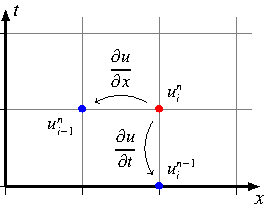
\includegraphics[width=\linewidth]{../BurgersEquation/tikz/quadratic/quadratic.pdf}\\
  \end{columns}
\end{frame}

\begin{frame}
  \begin{columns}
    \column{0.5\linewidth}
      Euler backwards
  $$\frac{u_{i}^{n}-u_{i}^{n-1}}{\Delta t}+ u_{i}^{n-1}\, \frac{u_{i}^{n}-u_{i-1}^{n}}{\Delta x}=0$$
  $$ u_{i}^{n} = \frac{u^{n-1}_{i}\, \left(\Delta{t}\, u^{n}_{i-1}\, + \Delta{x}\,\right)}{\Delta{t}\, u^{n-1}_{i}\, + \Delta{x}\,} $$
    \column{0.5\linewidth}
    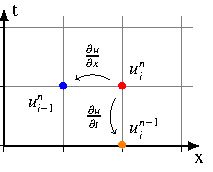
\includegraphics[width=\linewidth]{../BurgersEquation/tikz/linear5/linear5.pdf}\\
  \end{columns}
\end{frame}

\begin{frame}
  \frametitle{Implicit Euler method}
  \begin{columns}
    \column{0.6\linewidth}
    Euler backwards
    $$\frac{u_{i}^{n}-u_{i}^{n-1}}{\Delta t}+ u_{i}^{n-1}\, \frac{u_{i+1}^{n}-u_{i-1}^{n}}{2\,\Delta x}=0$$
$$-u_{i}^{n-1} \, dt \, u_{i-1}^{n} +  2 \, dx \,  u_{i}^{n} + u_{i}^{n-1} \, dt \, u_{i+1}^{n}=  2 \, dx \, u_{i}^{n-1}$$
    \column{0.4\linewidth}
    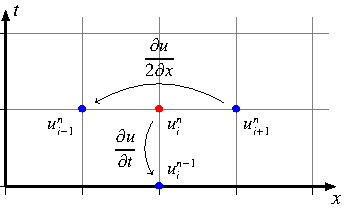
\includegraphics[width=\linewidth]{../BurgersEquation/tikz/implicit/implicit.pdf}\\
  \end{columns}
\end{frame}

\begin{frame}
  \frametitle{Implicit Euler method}
  $$-u_{i}^{n-1} \, dt \, u_{i-1}^{n} +  2 \, dx \,  u_{i}^{n} + u_{i}^{n-1} \, dt \, u_{i+1}^{n}=  2 \, dx \, u_{i}^{n-1}$$

  $$  \left[{\begin{matrix}
    {dx- u_{1}^{n}\, dt}&{ u_{1}^{n} \, dt}&{0}&{}&{0}\\[5pt]
    {-u_{2}^{n} \, dt}&{ 2 \, dx}&{ u_{2}^{n} \, dt}&{}&{0}\\[5pt]
    {0}&{-u_{3}^{n} \, dt}&{ 2 \, dx}&\ddots &{0}\\[5pt]
    {0}&{0}&\ddots &\ddots &{ u_{M-1}^{n} \, dt}\\[5pt]
    {0}&{0}&{}&{-u_{M}^{n} \, dt}&{dx + u_{1}^{M}\, dt}
    \end{matrix}}
    \right]\left[{
    \begin{matrix}
    { u_{1}^{n+1}}\\[5pt]
    { u_{2}^{n+1}}\\[5pt]
    { u_{3}^{n+1}}\\[5pt]
    \vdots \\[5pt]
    { u_{M}^{n+1}}
    \end{matrix}}
    \right]
    =\left[{
    \begin{matrix}
    {dx \, u_{1}^{n}}\\[5pt]
    { 2 \, dx \, u_{2}^{n}}\\[5pt]
    { 2 \, dx \, u_{3}^{n}}\\[5pt]
    \vdots \\[5pt]
    {dx \, u_{M}^{n}}
    \end{matrix}}
    \right]$$
\end{frame}


\begin{frame}
  $$a_{i}x_{{i-1}}+b_{i}x_{i}+c_{i}x_{{i+1}}=d_{i}$$
  $$\begin{bmatrix}{b_{1}}&{c_{1}}&{}&{}&{0}\\
      {a_{2}}&{b_{2}}&{c_{2}}&{}&{}\\
      {}&{a_{3}}&{b_{3}}&\ddots &{}\\
      {}&{}&\ddots &\ddots &{c_{n-1}}\\
      {0}&{}&{}&{a_{n}}&{b_{n}}\\
      \end{bmatrix}
      \begin{bmatrix}{x_{1}}\\
      {x_{2}}\\{x_{3}}\\\vdots \\
      {x_{n}}\\
      \end{bmatrix}
      =
      \begin{bmatrix}{d_{1}}\\
      {d_{2}}\\{d_{3}}\\
      \vdots \\{d_{n}}\\
    \end{bmatrix} $$
\end{frame}

\begin{frame}
\begin{center}
  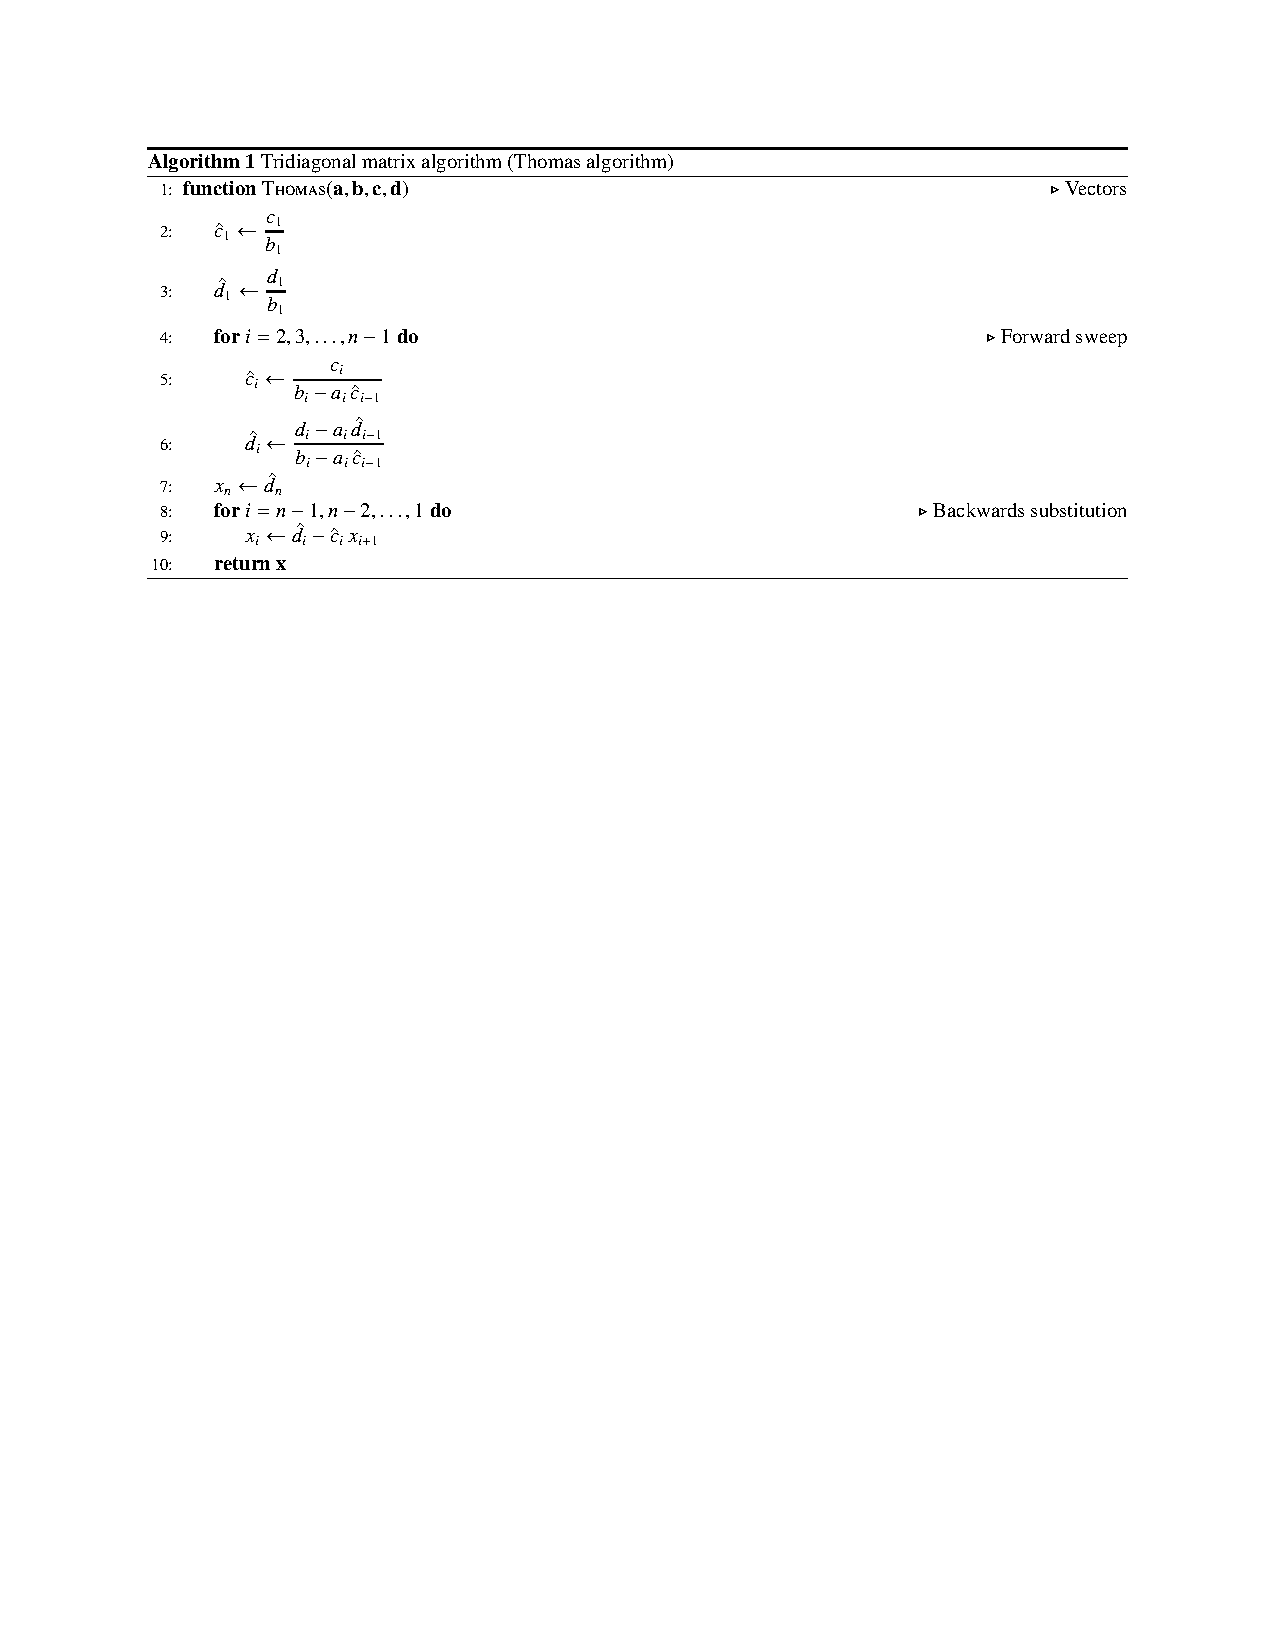
\includegraphics[width=.9\linewidth]{../BurgersEquation/tex/implicit/algo_cropped.pdf}\\
\end{center}
\end{frame}

% 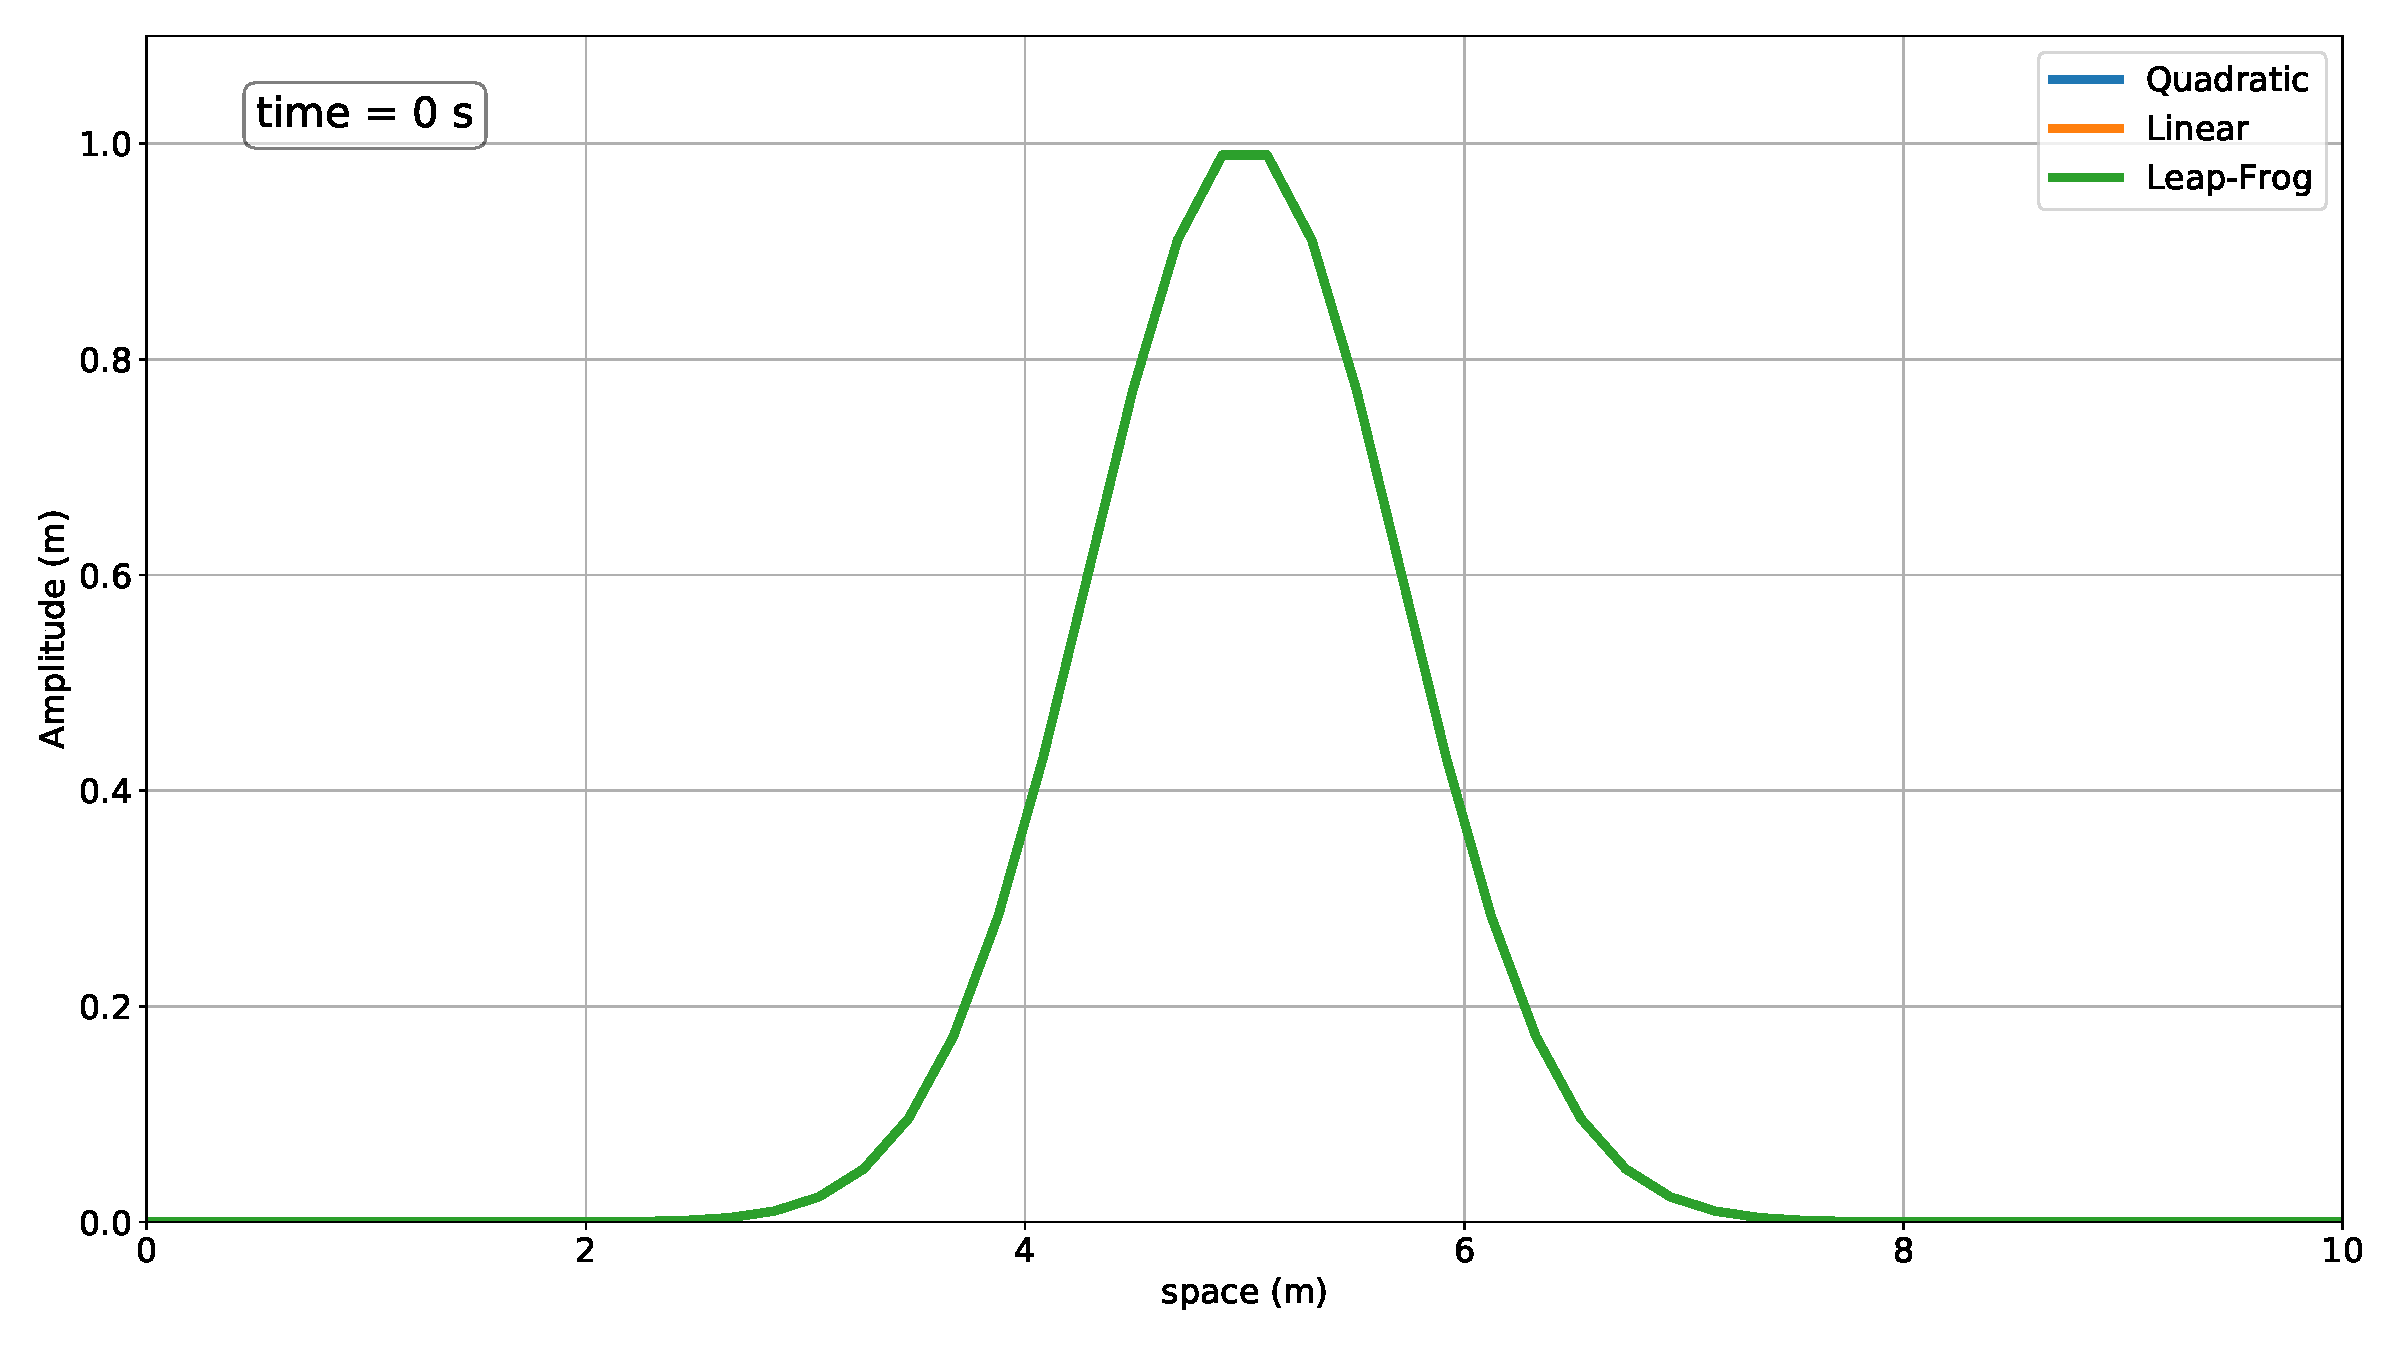
\includegraphics[width=\linewidth]{../BurgersEquation/images/imp0.pdf}
% 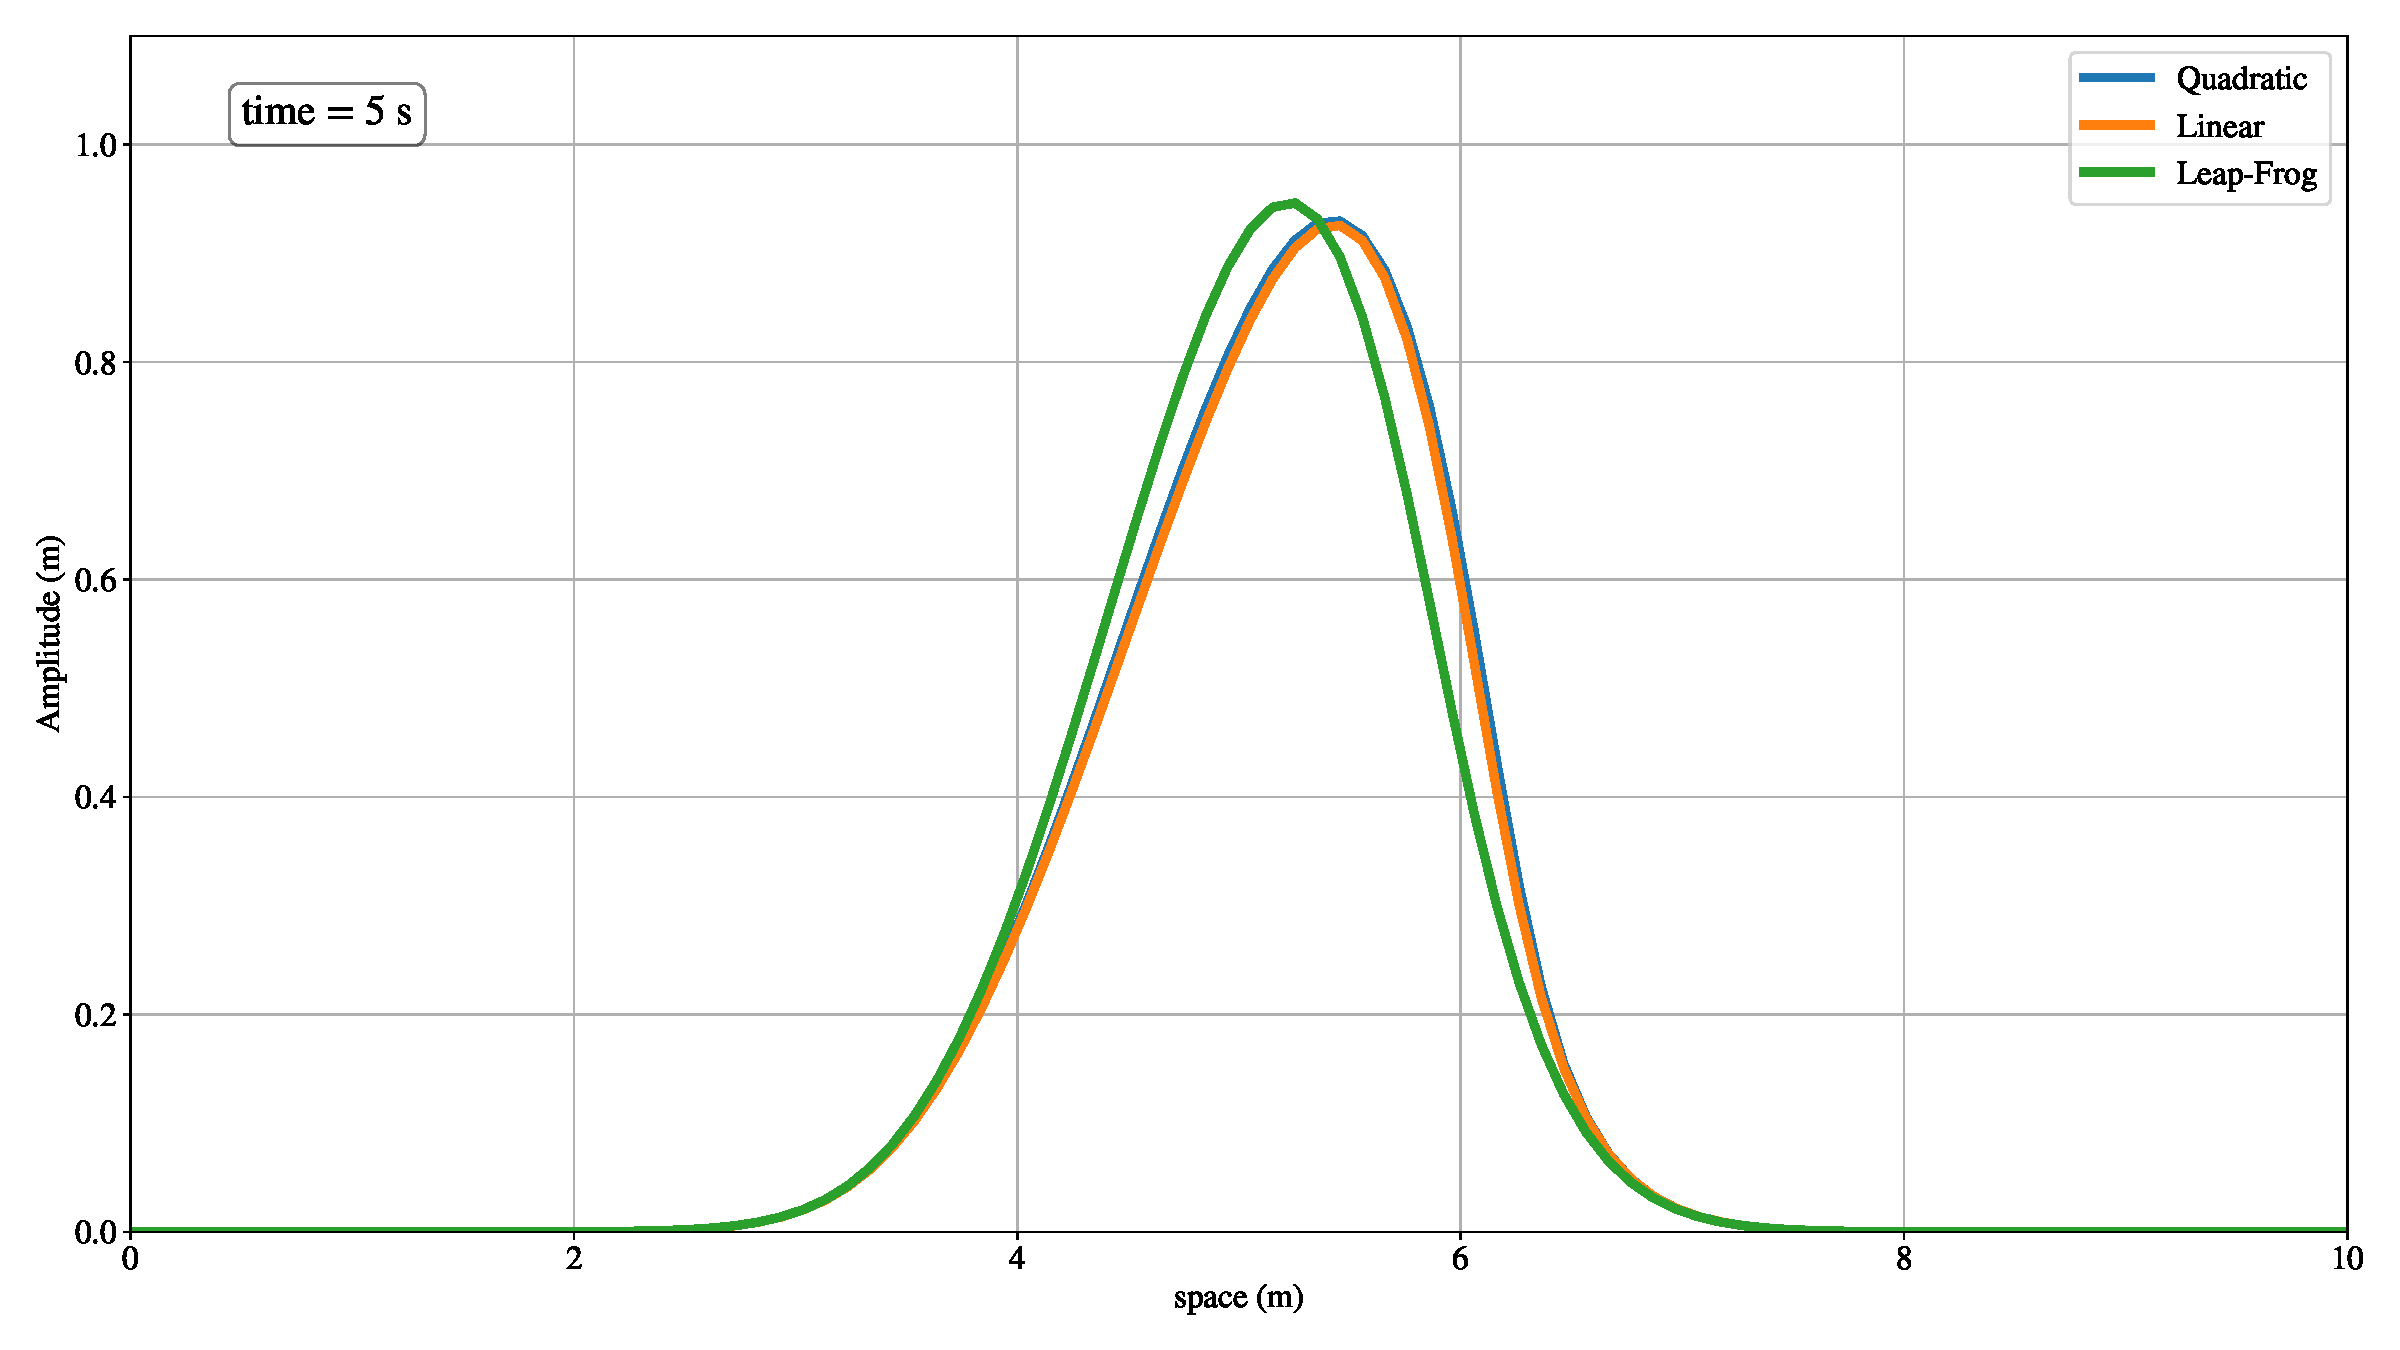
\includegraphics[width=\linewidth]{../BurgersEquation/images/imp1.pdf}
% 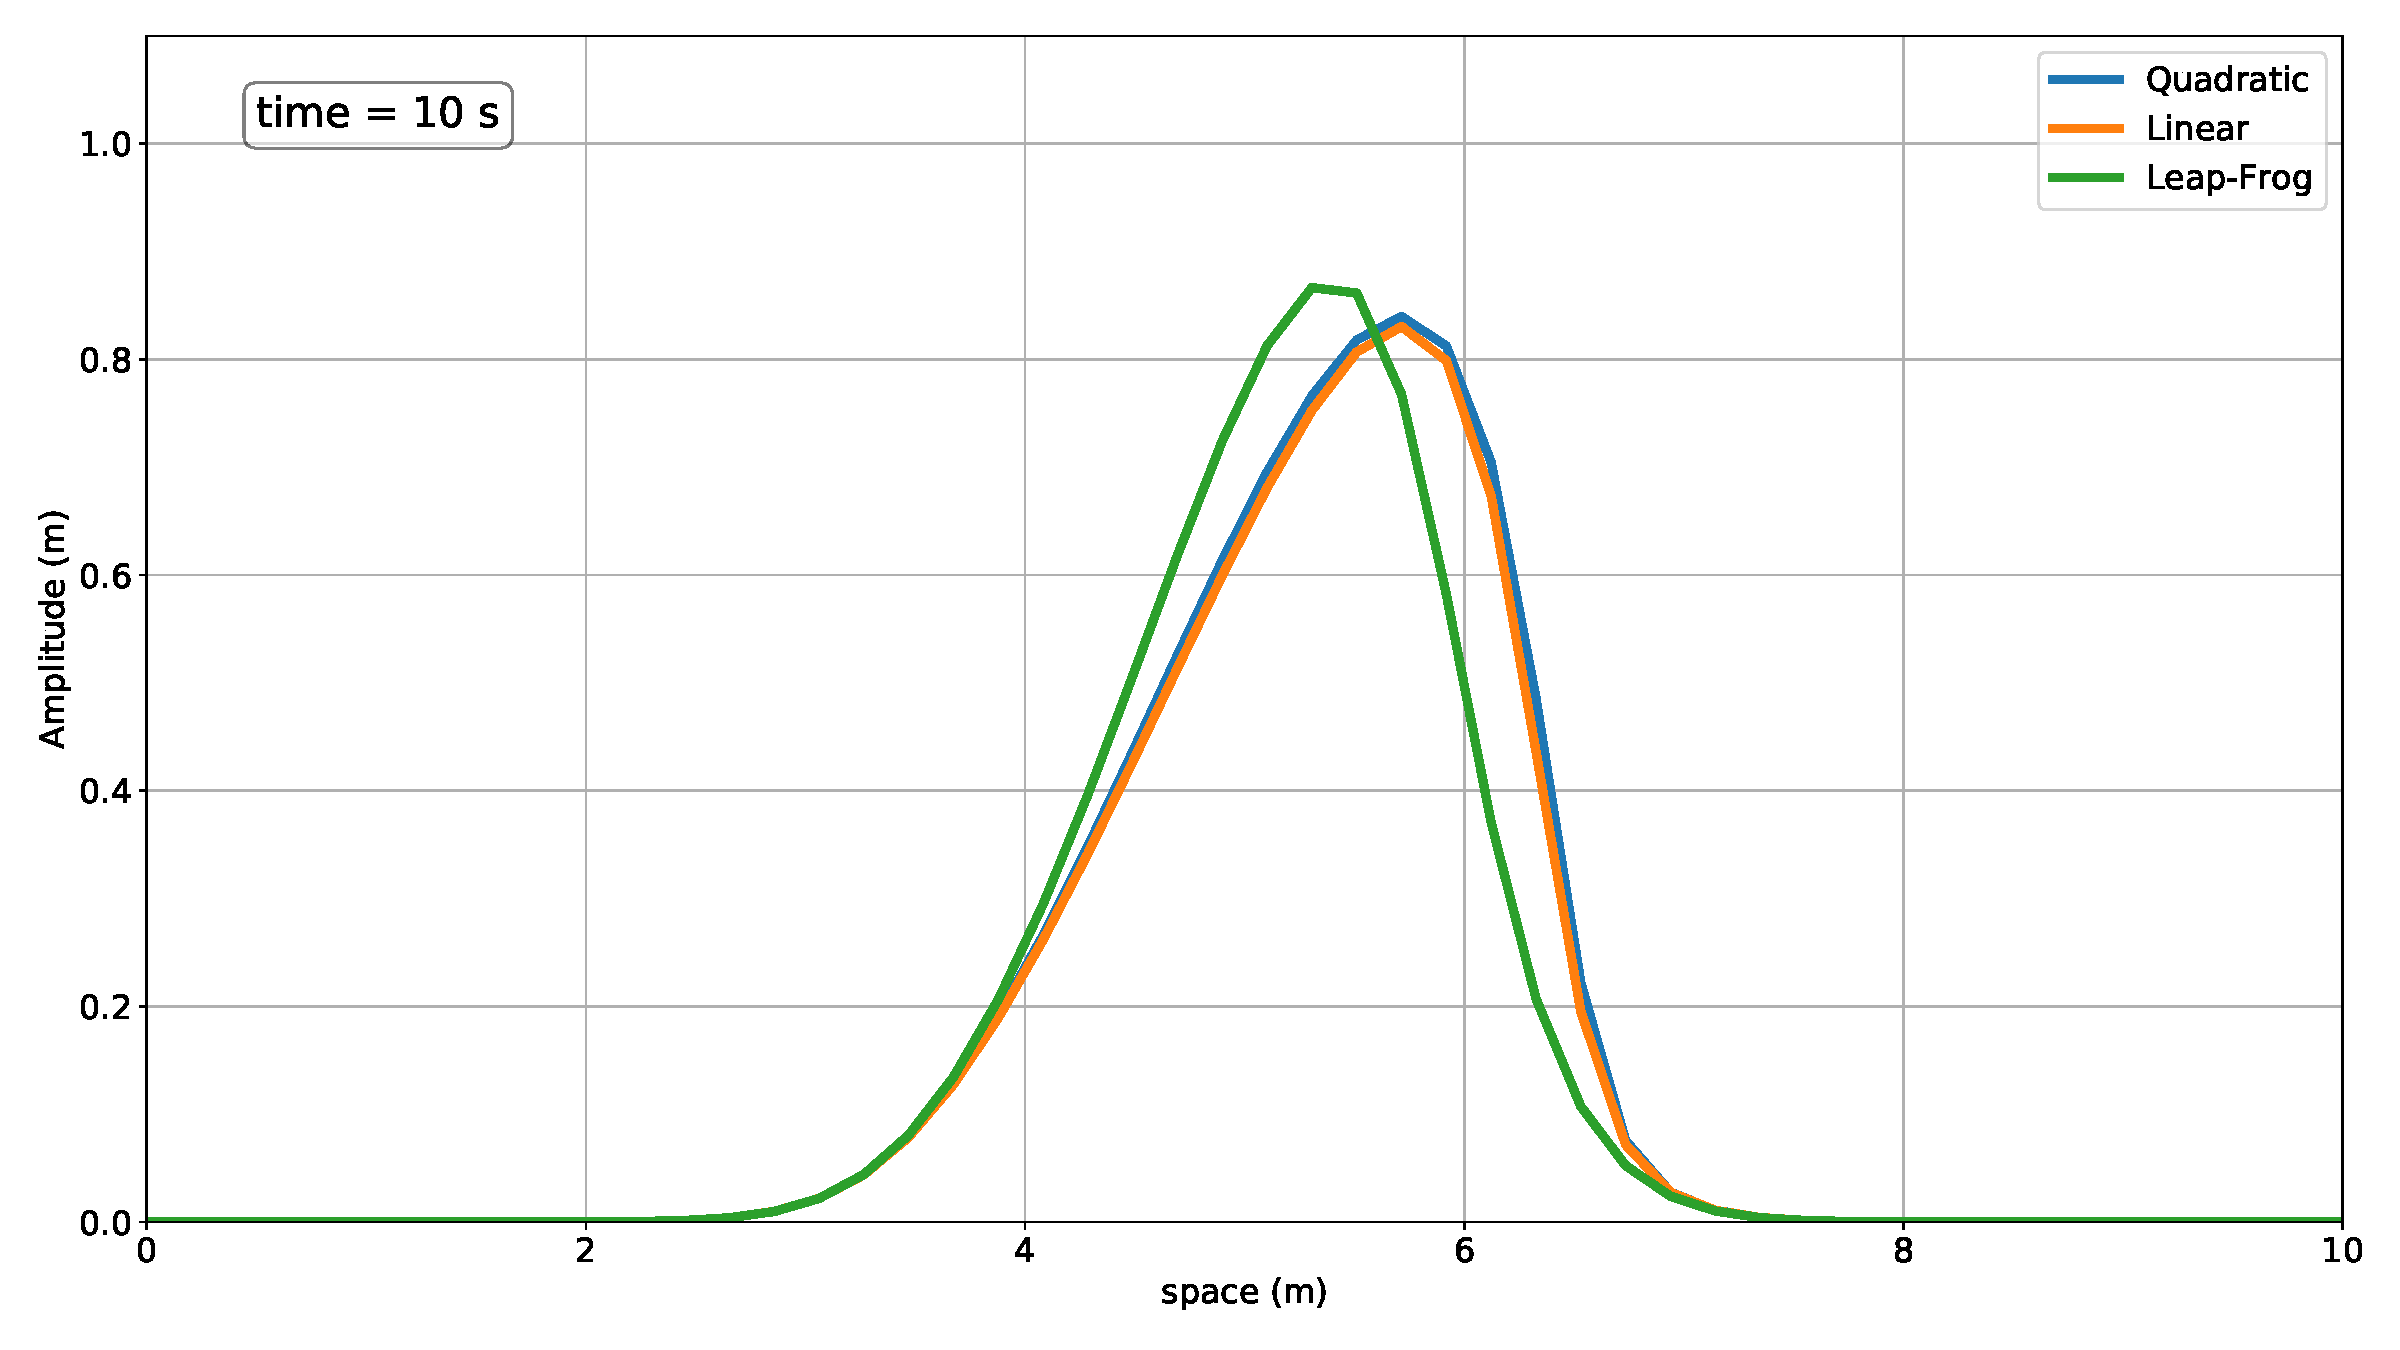
\includegraphics[width=\linewidth]{../BurgersEquation/images/imp2.pdf}
% 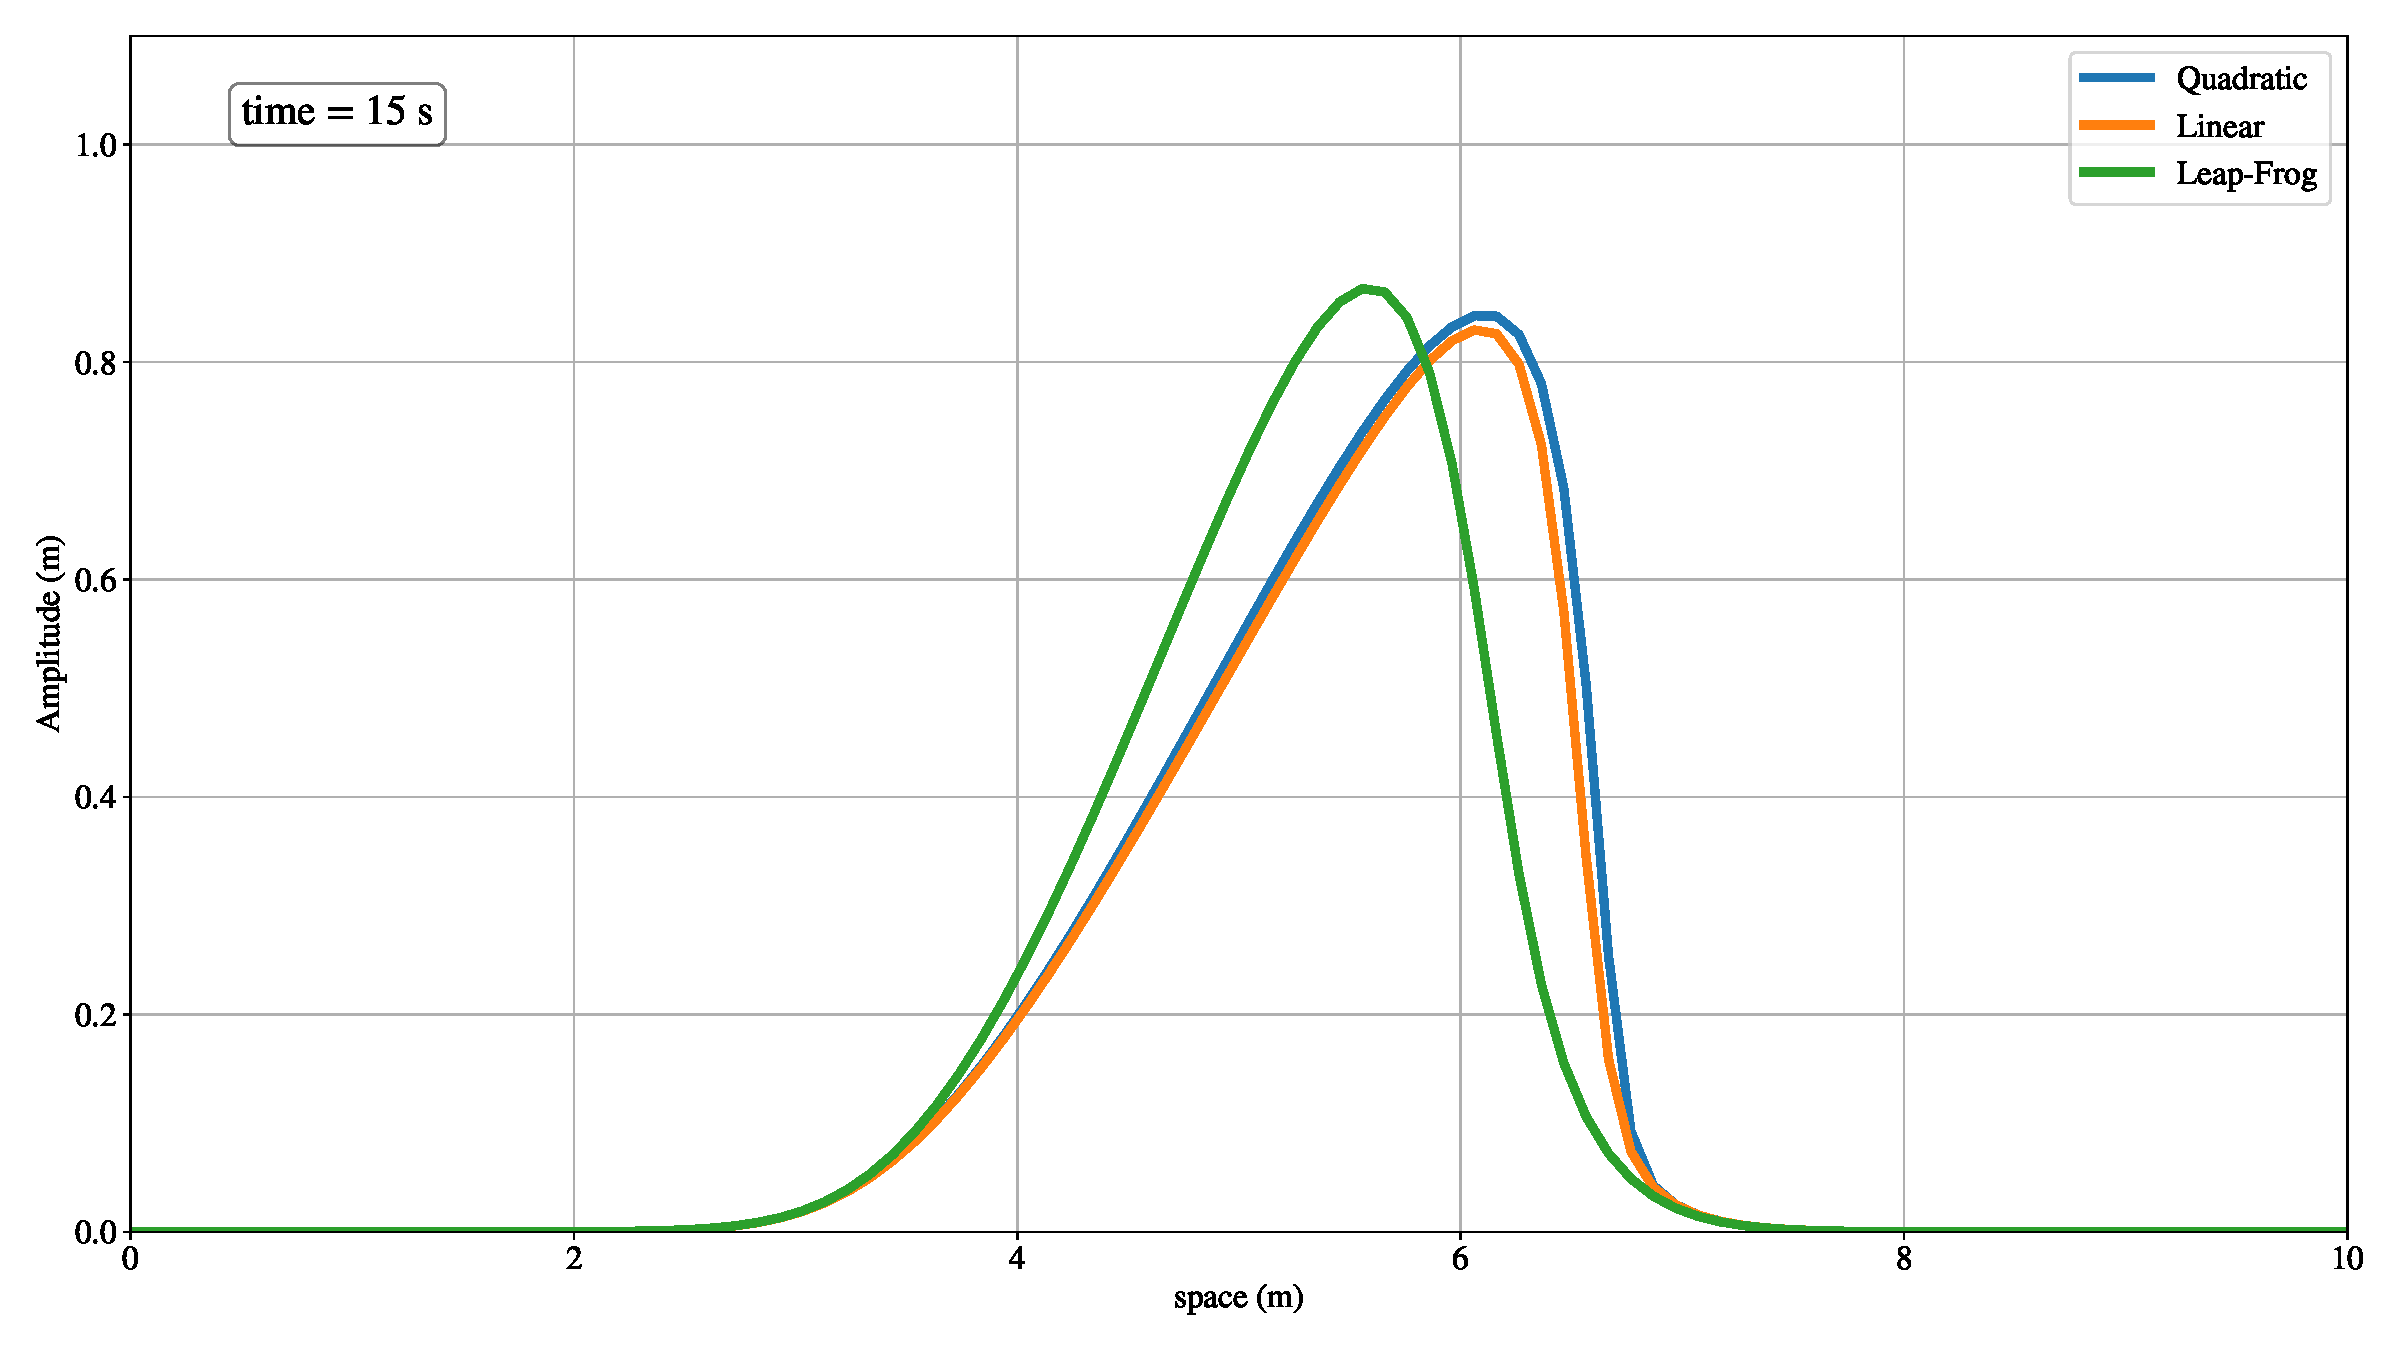
\includegraphics[width=\linewidth]{../BurgersEquation/images/imp3.pdf}
% 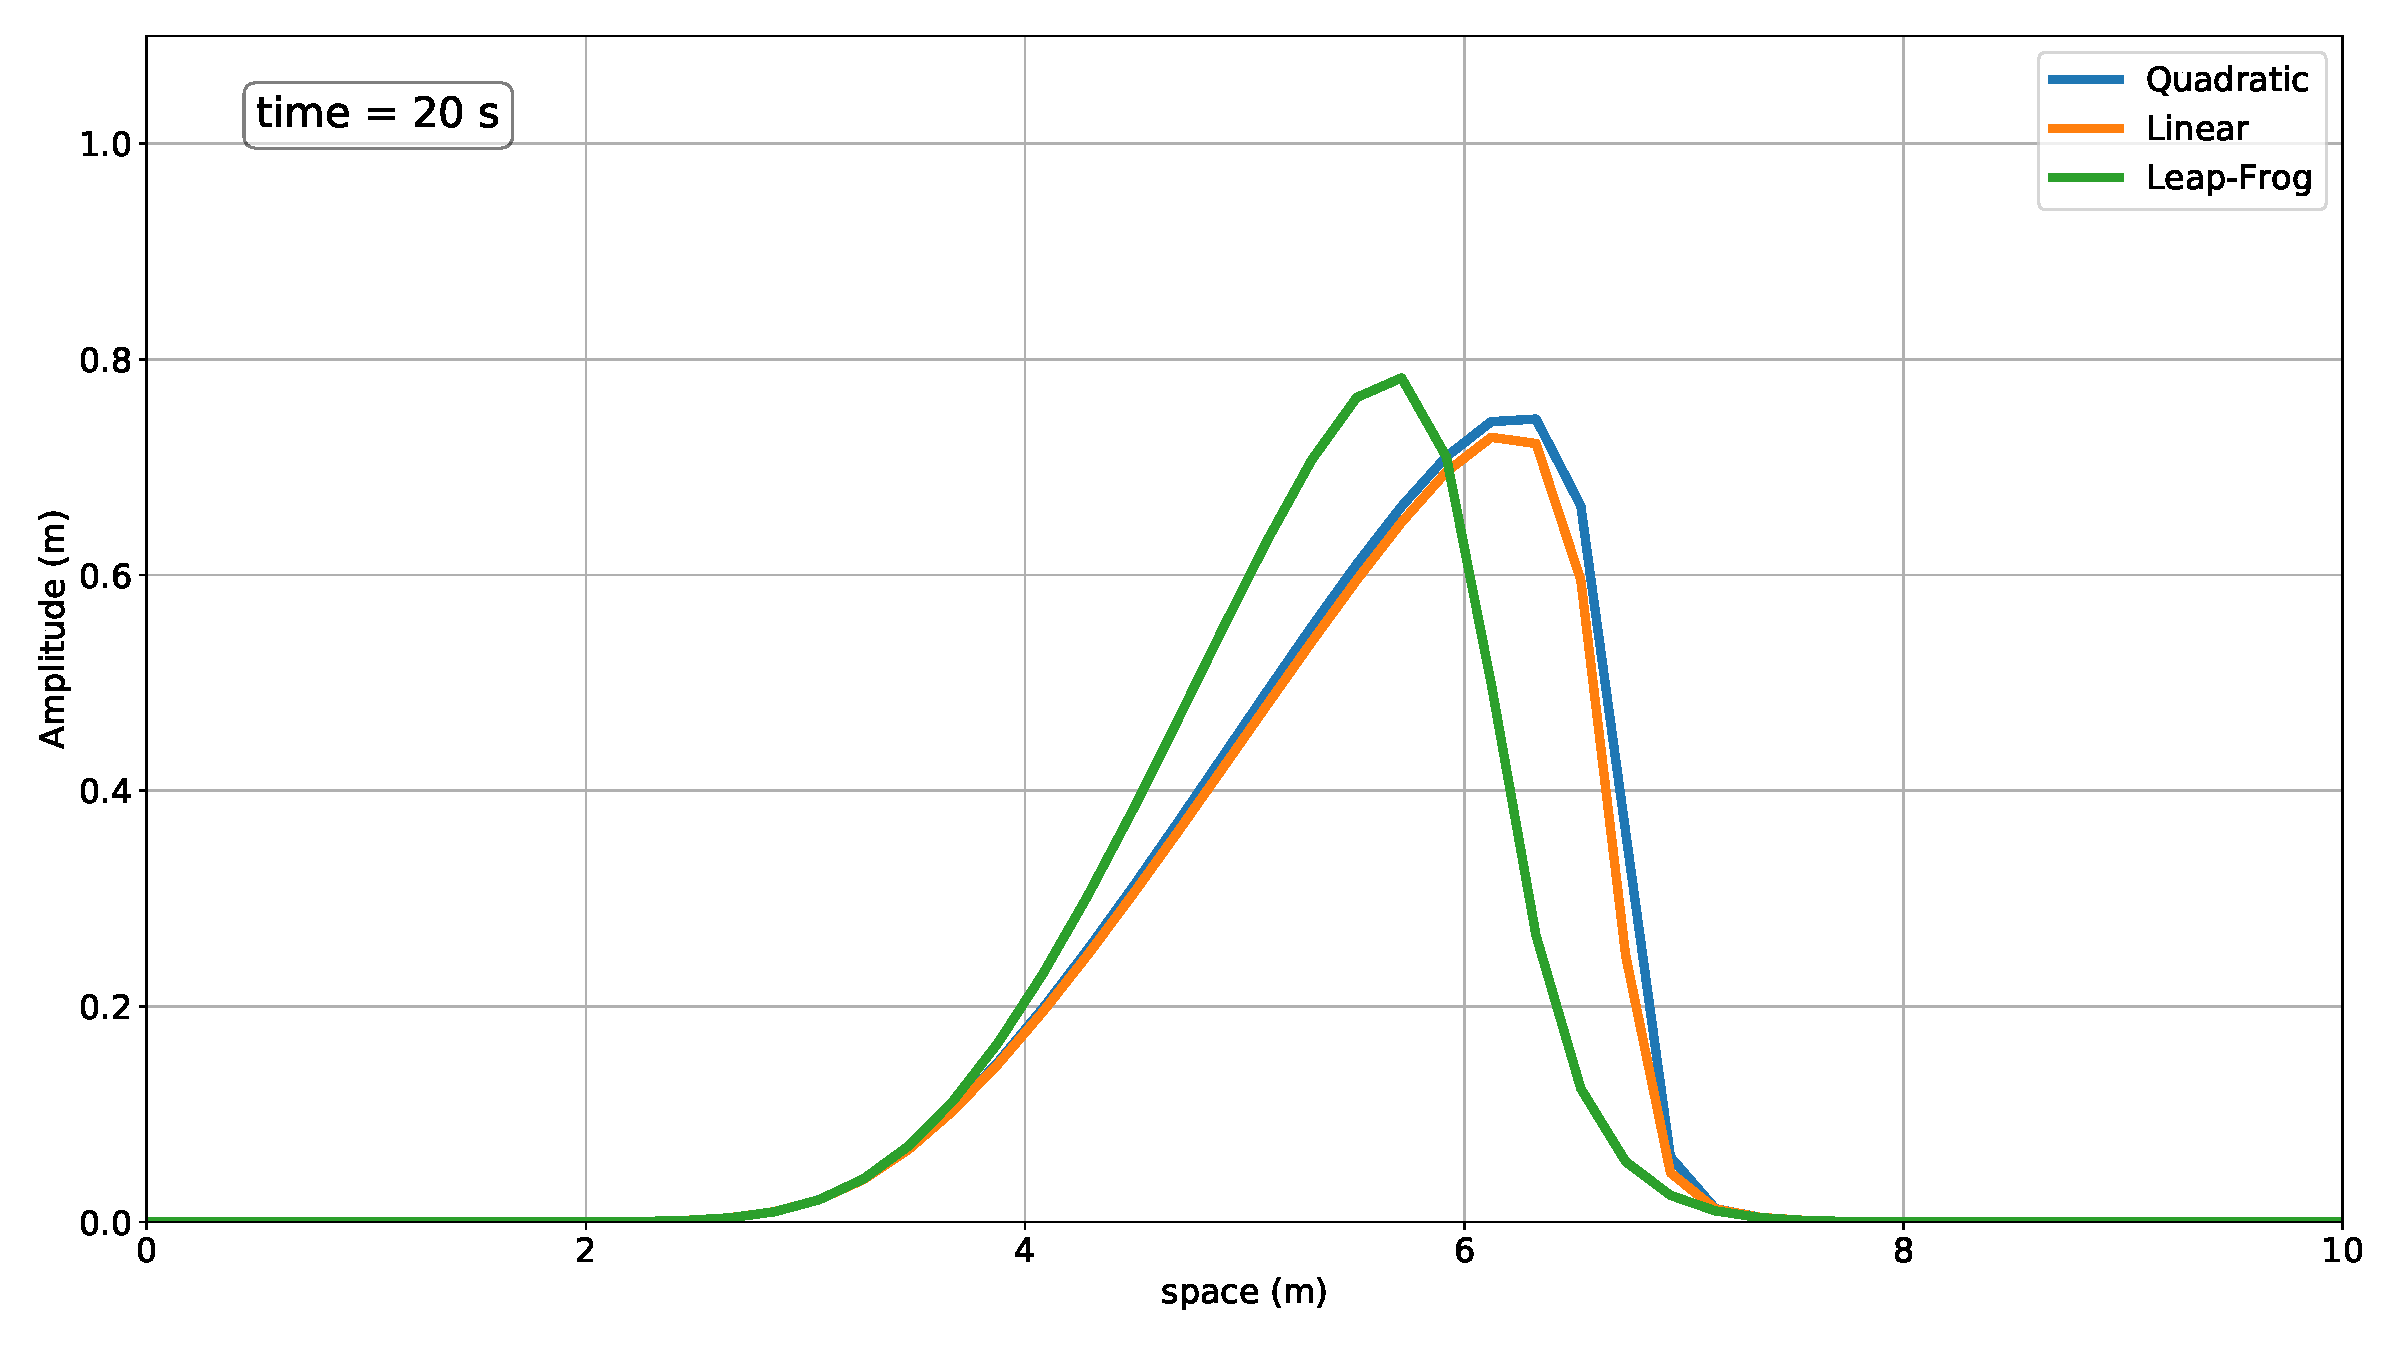
\includegraphics[width=\linewidth]{../BurgersEquation/images/imp4.pdf}
% 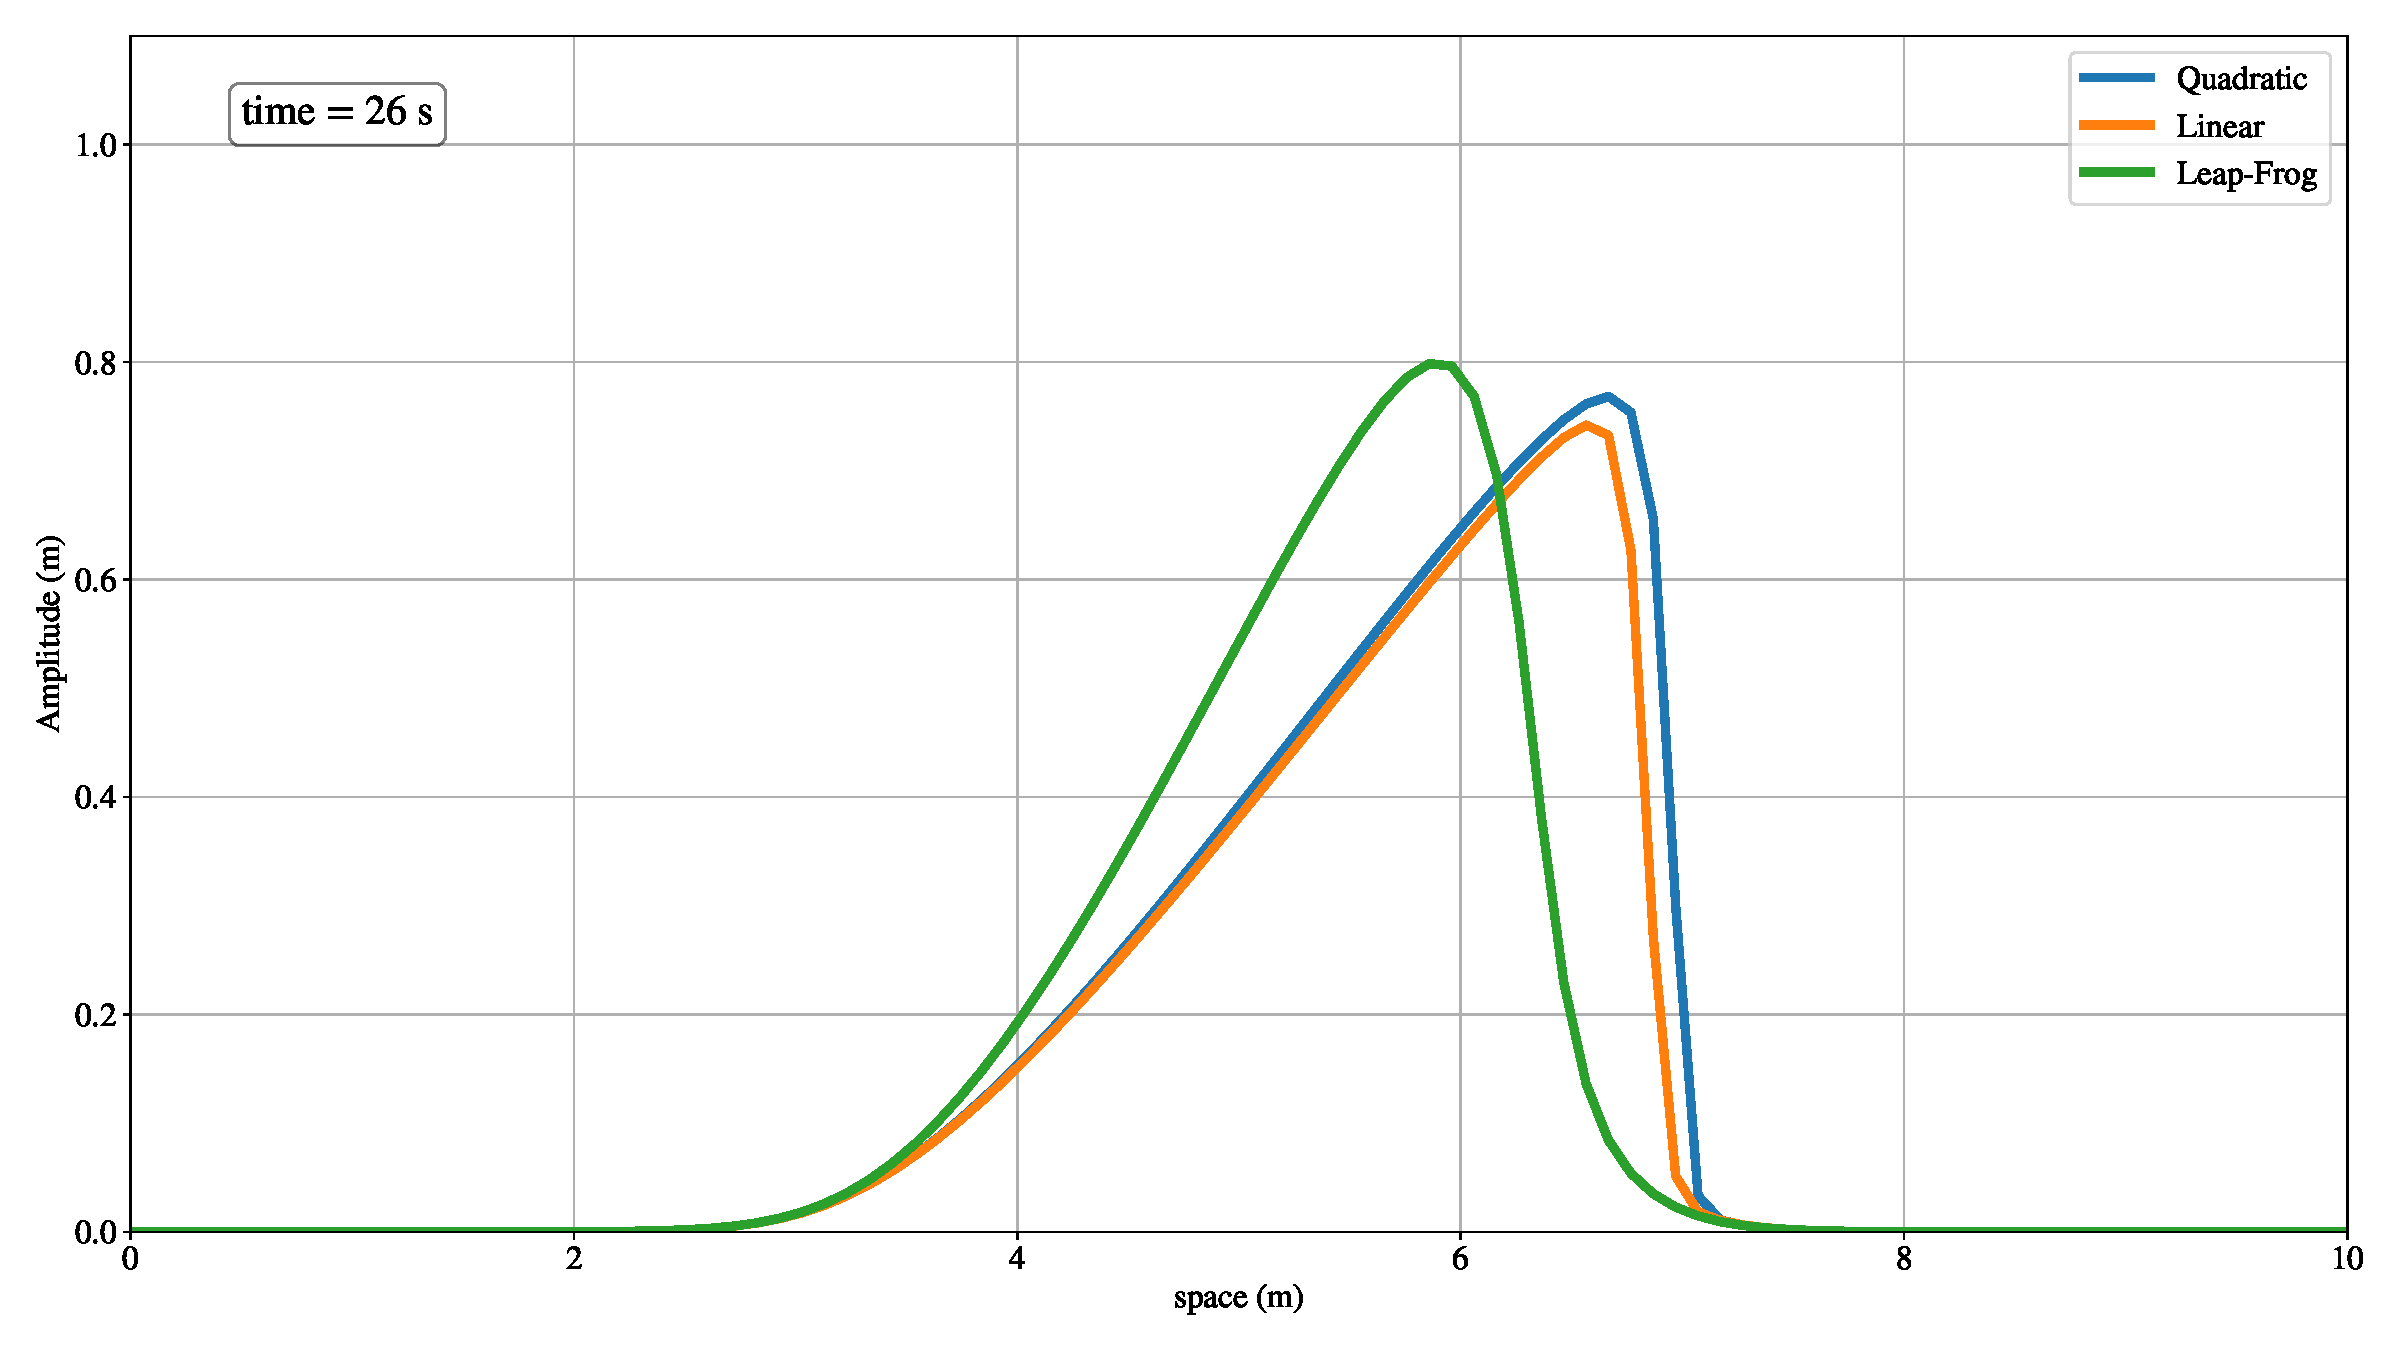
\includegraphics[width=\linewidth]{../BurgersEquation/images/imp5.pdf}
% 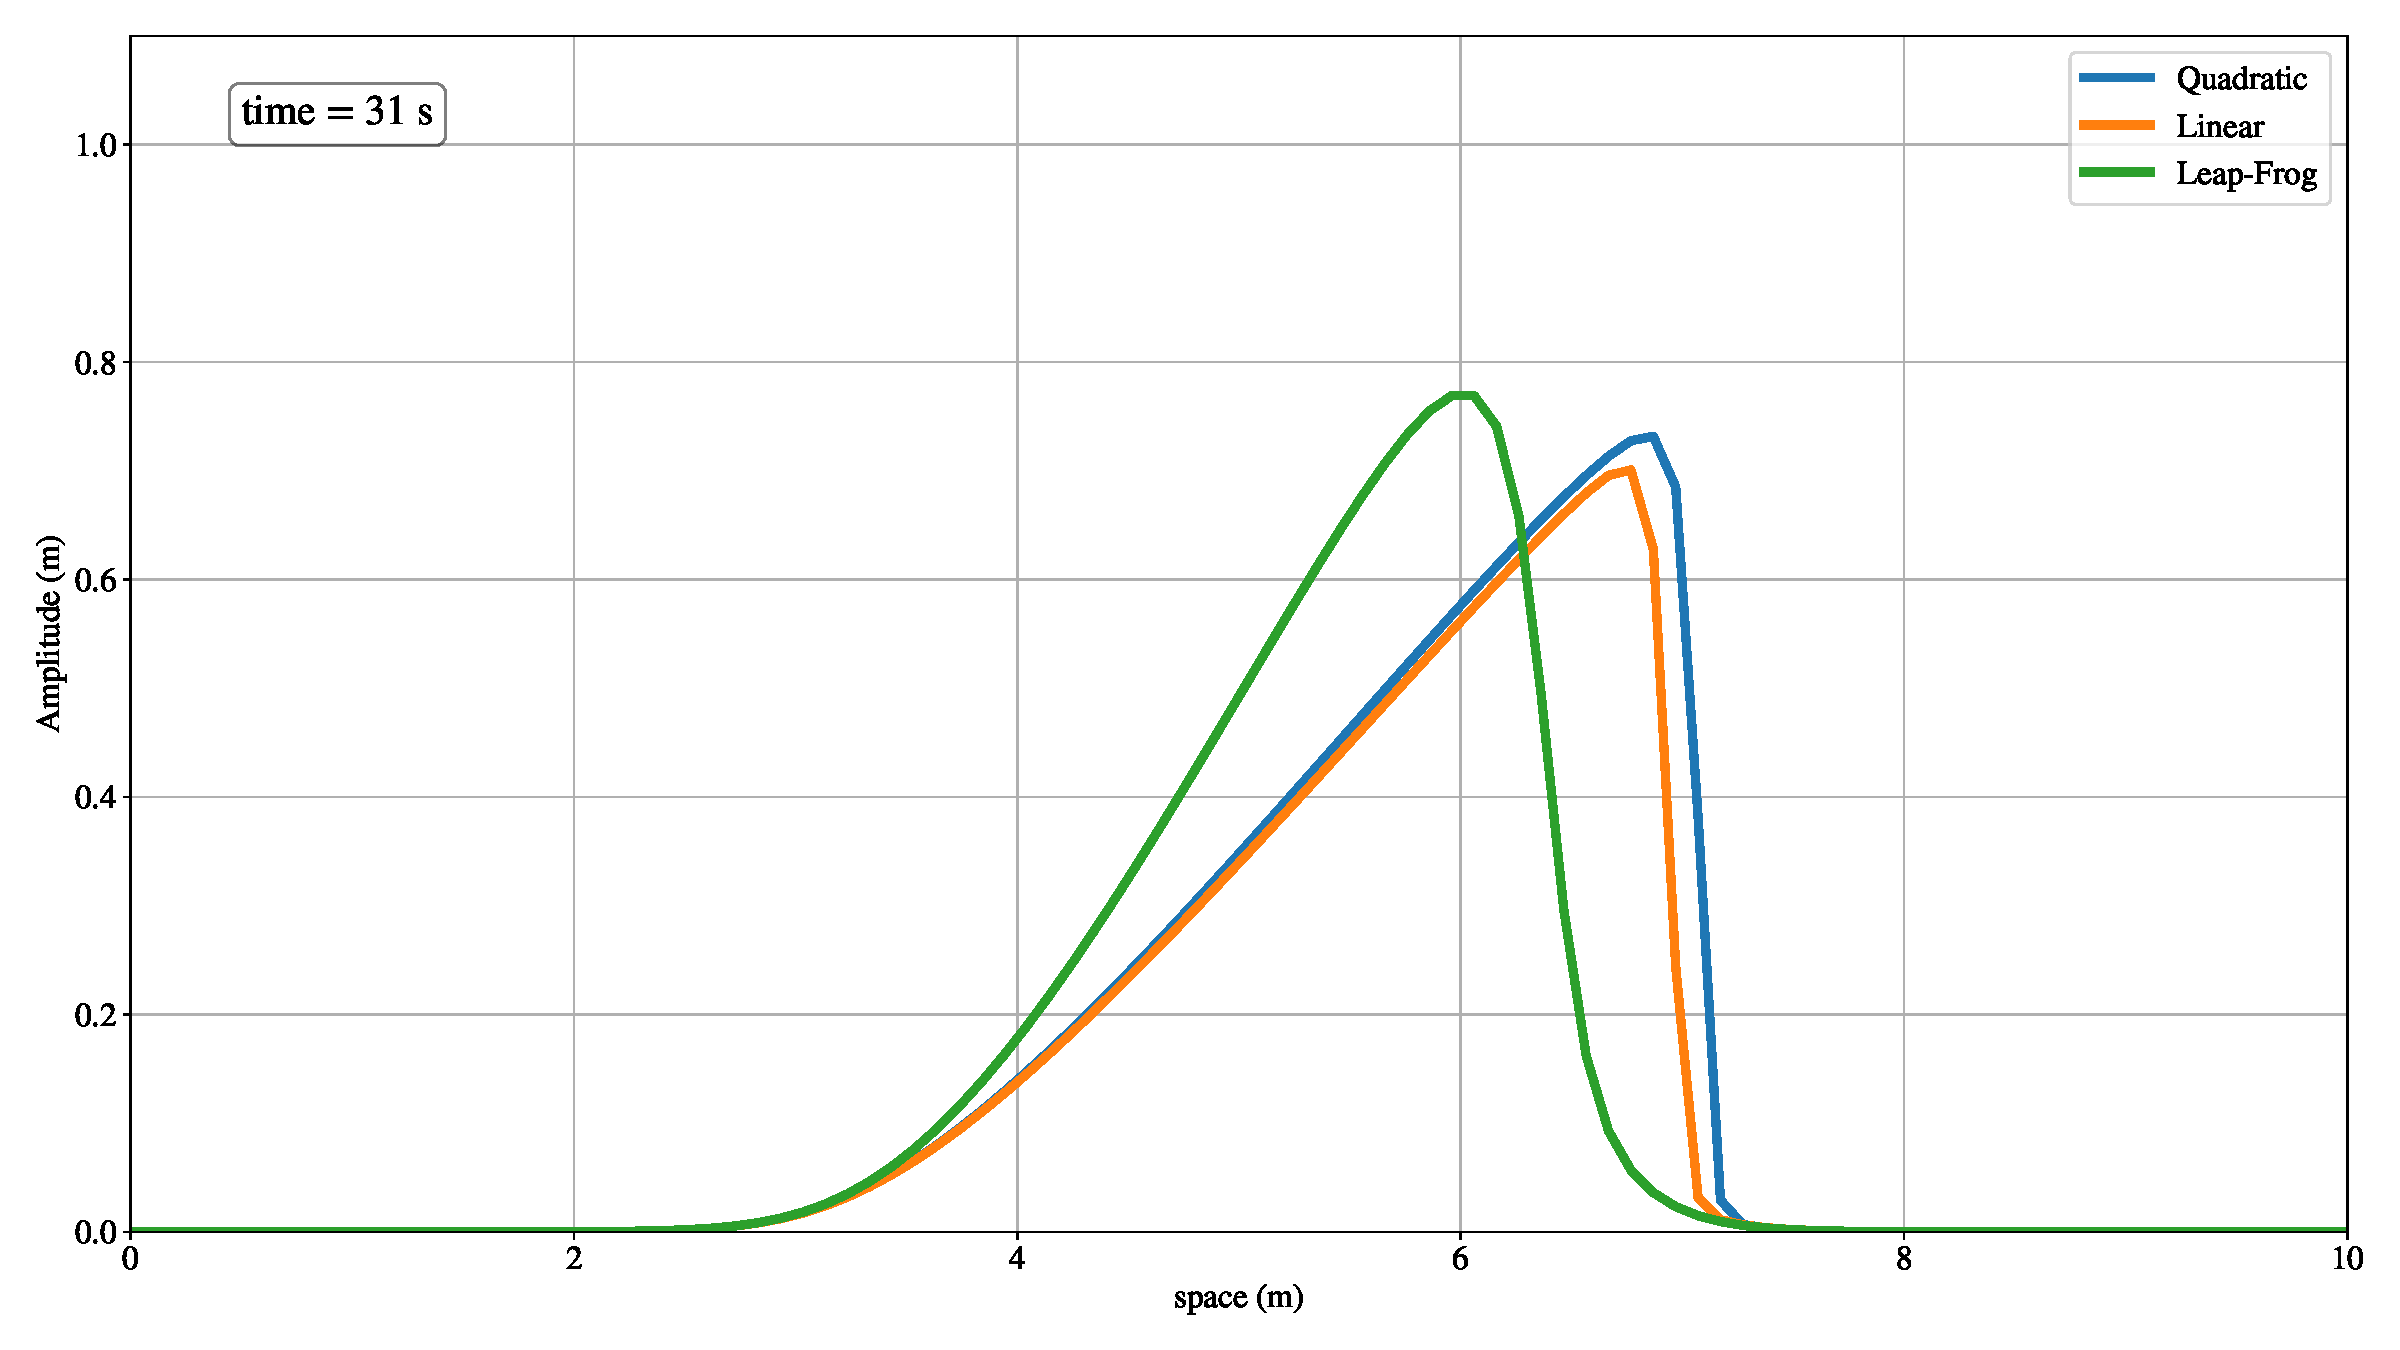
\includegraphics[width=\linewidth]{../BurgersEquation/images/imp6.pdf}
% 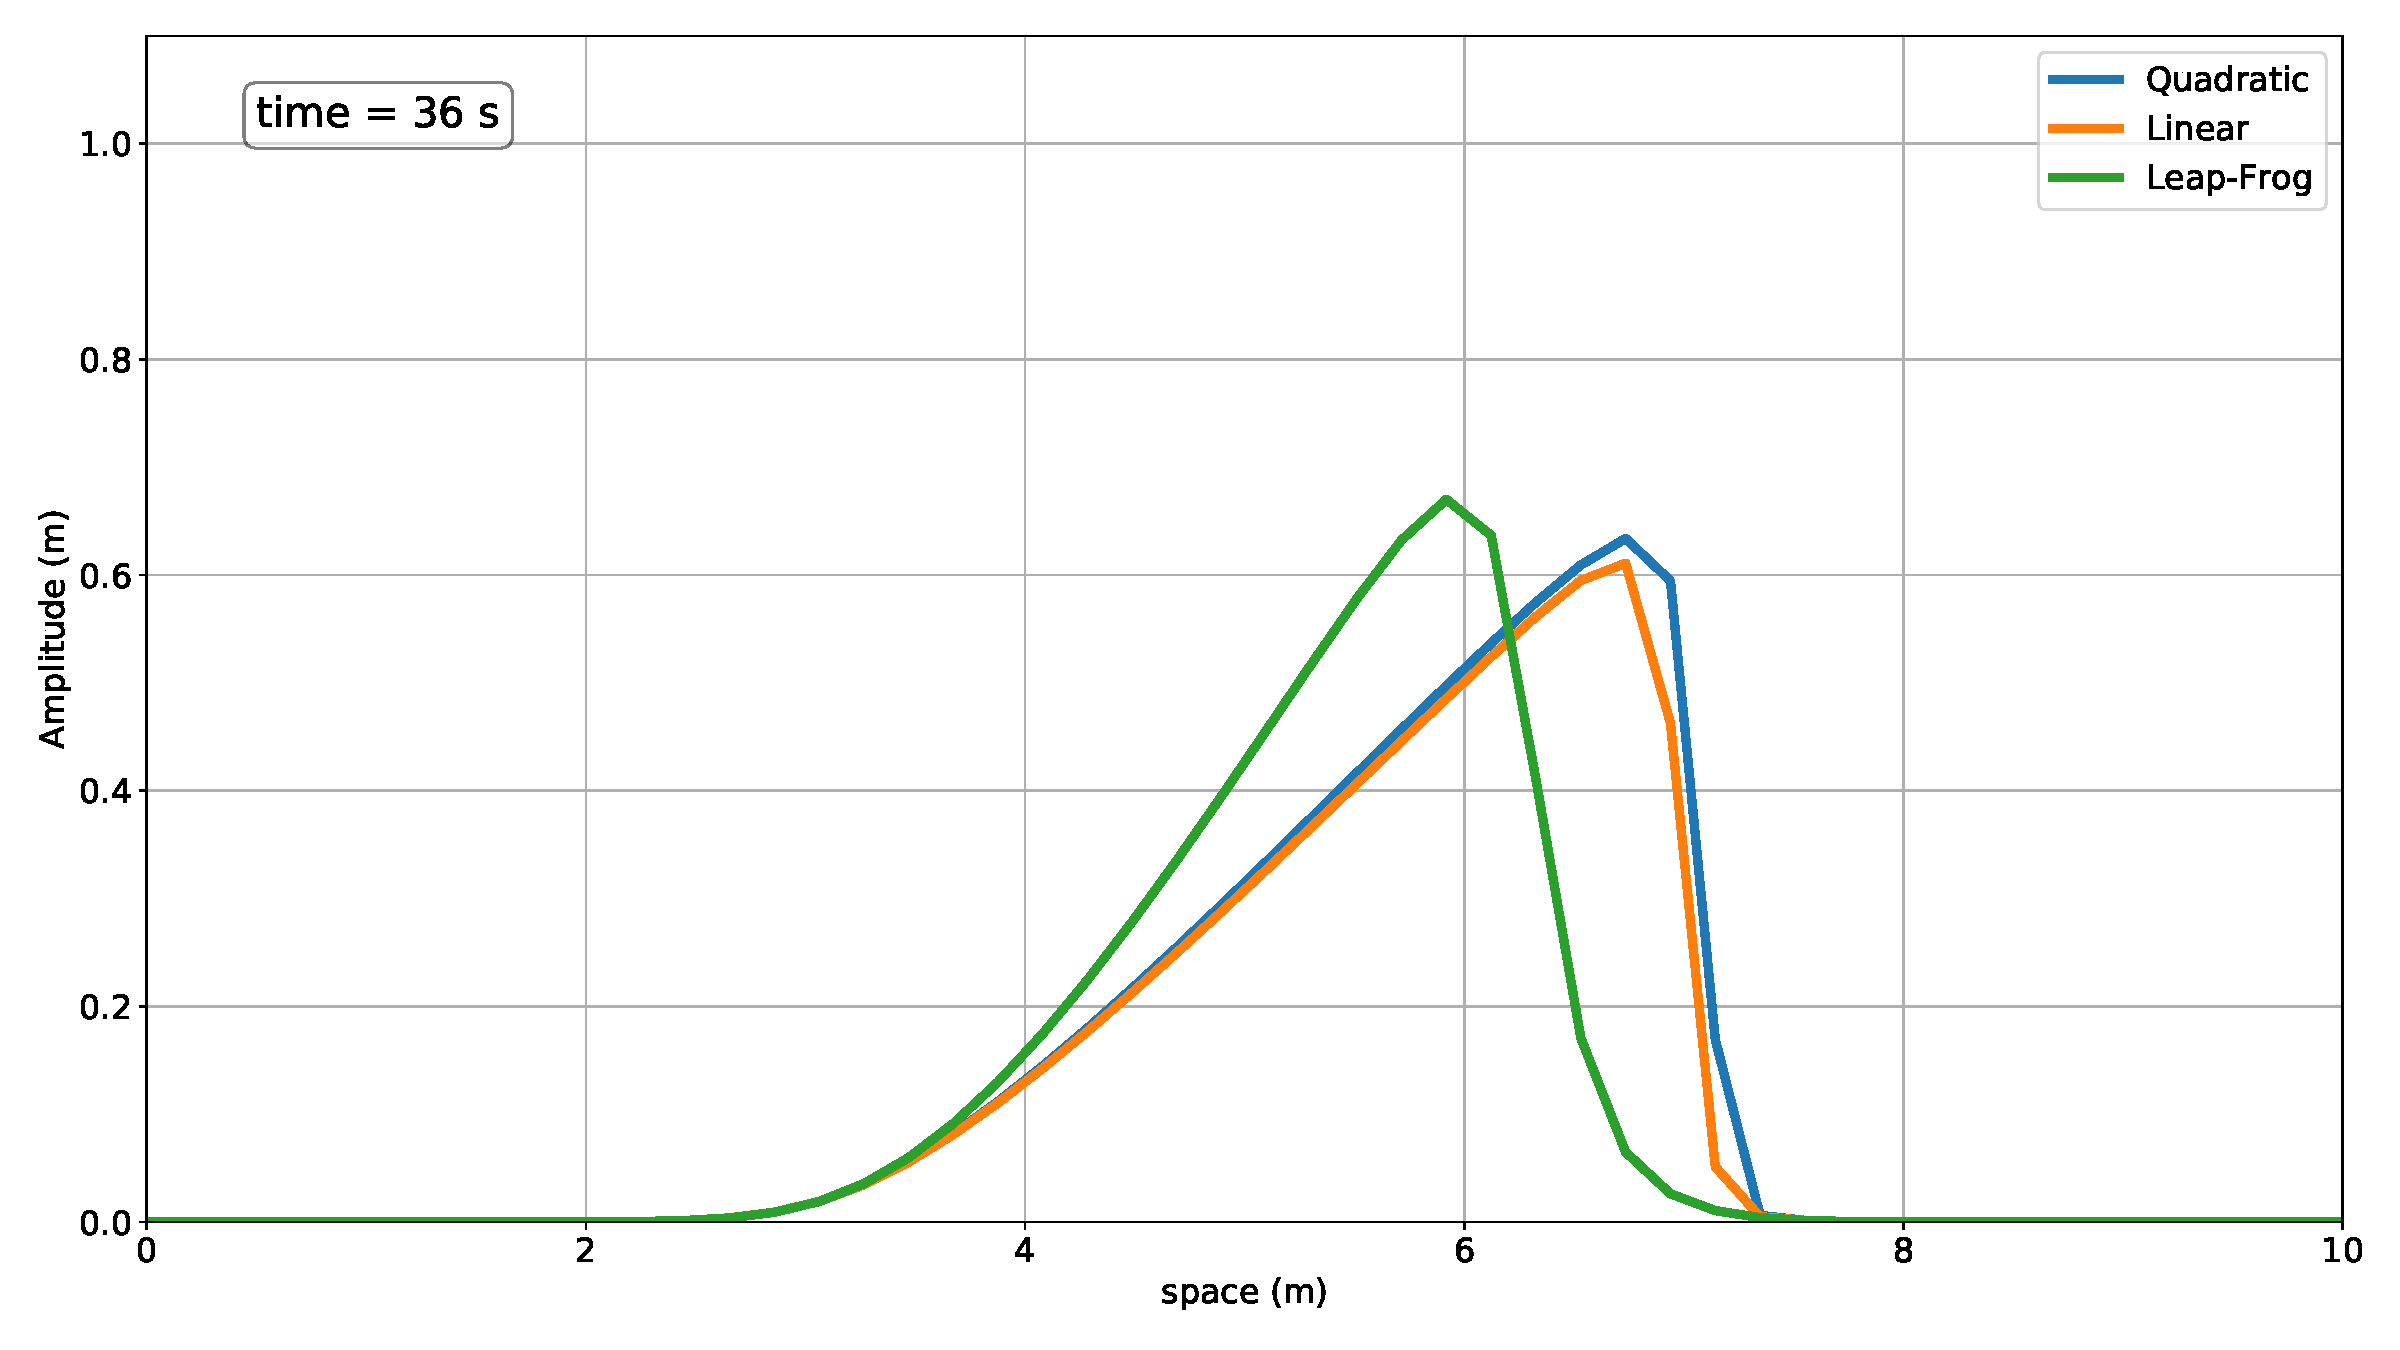
\includegraphics[width=\linewidth]{../BurgersEquation/images/imp7.pdf}
% 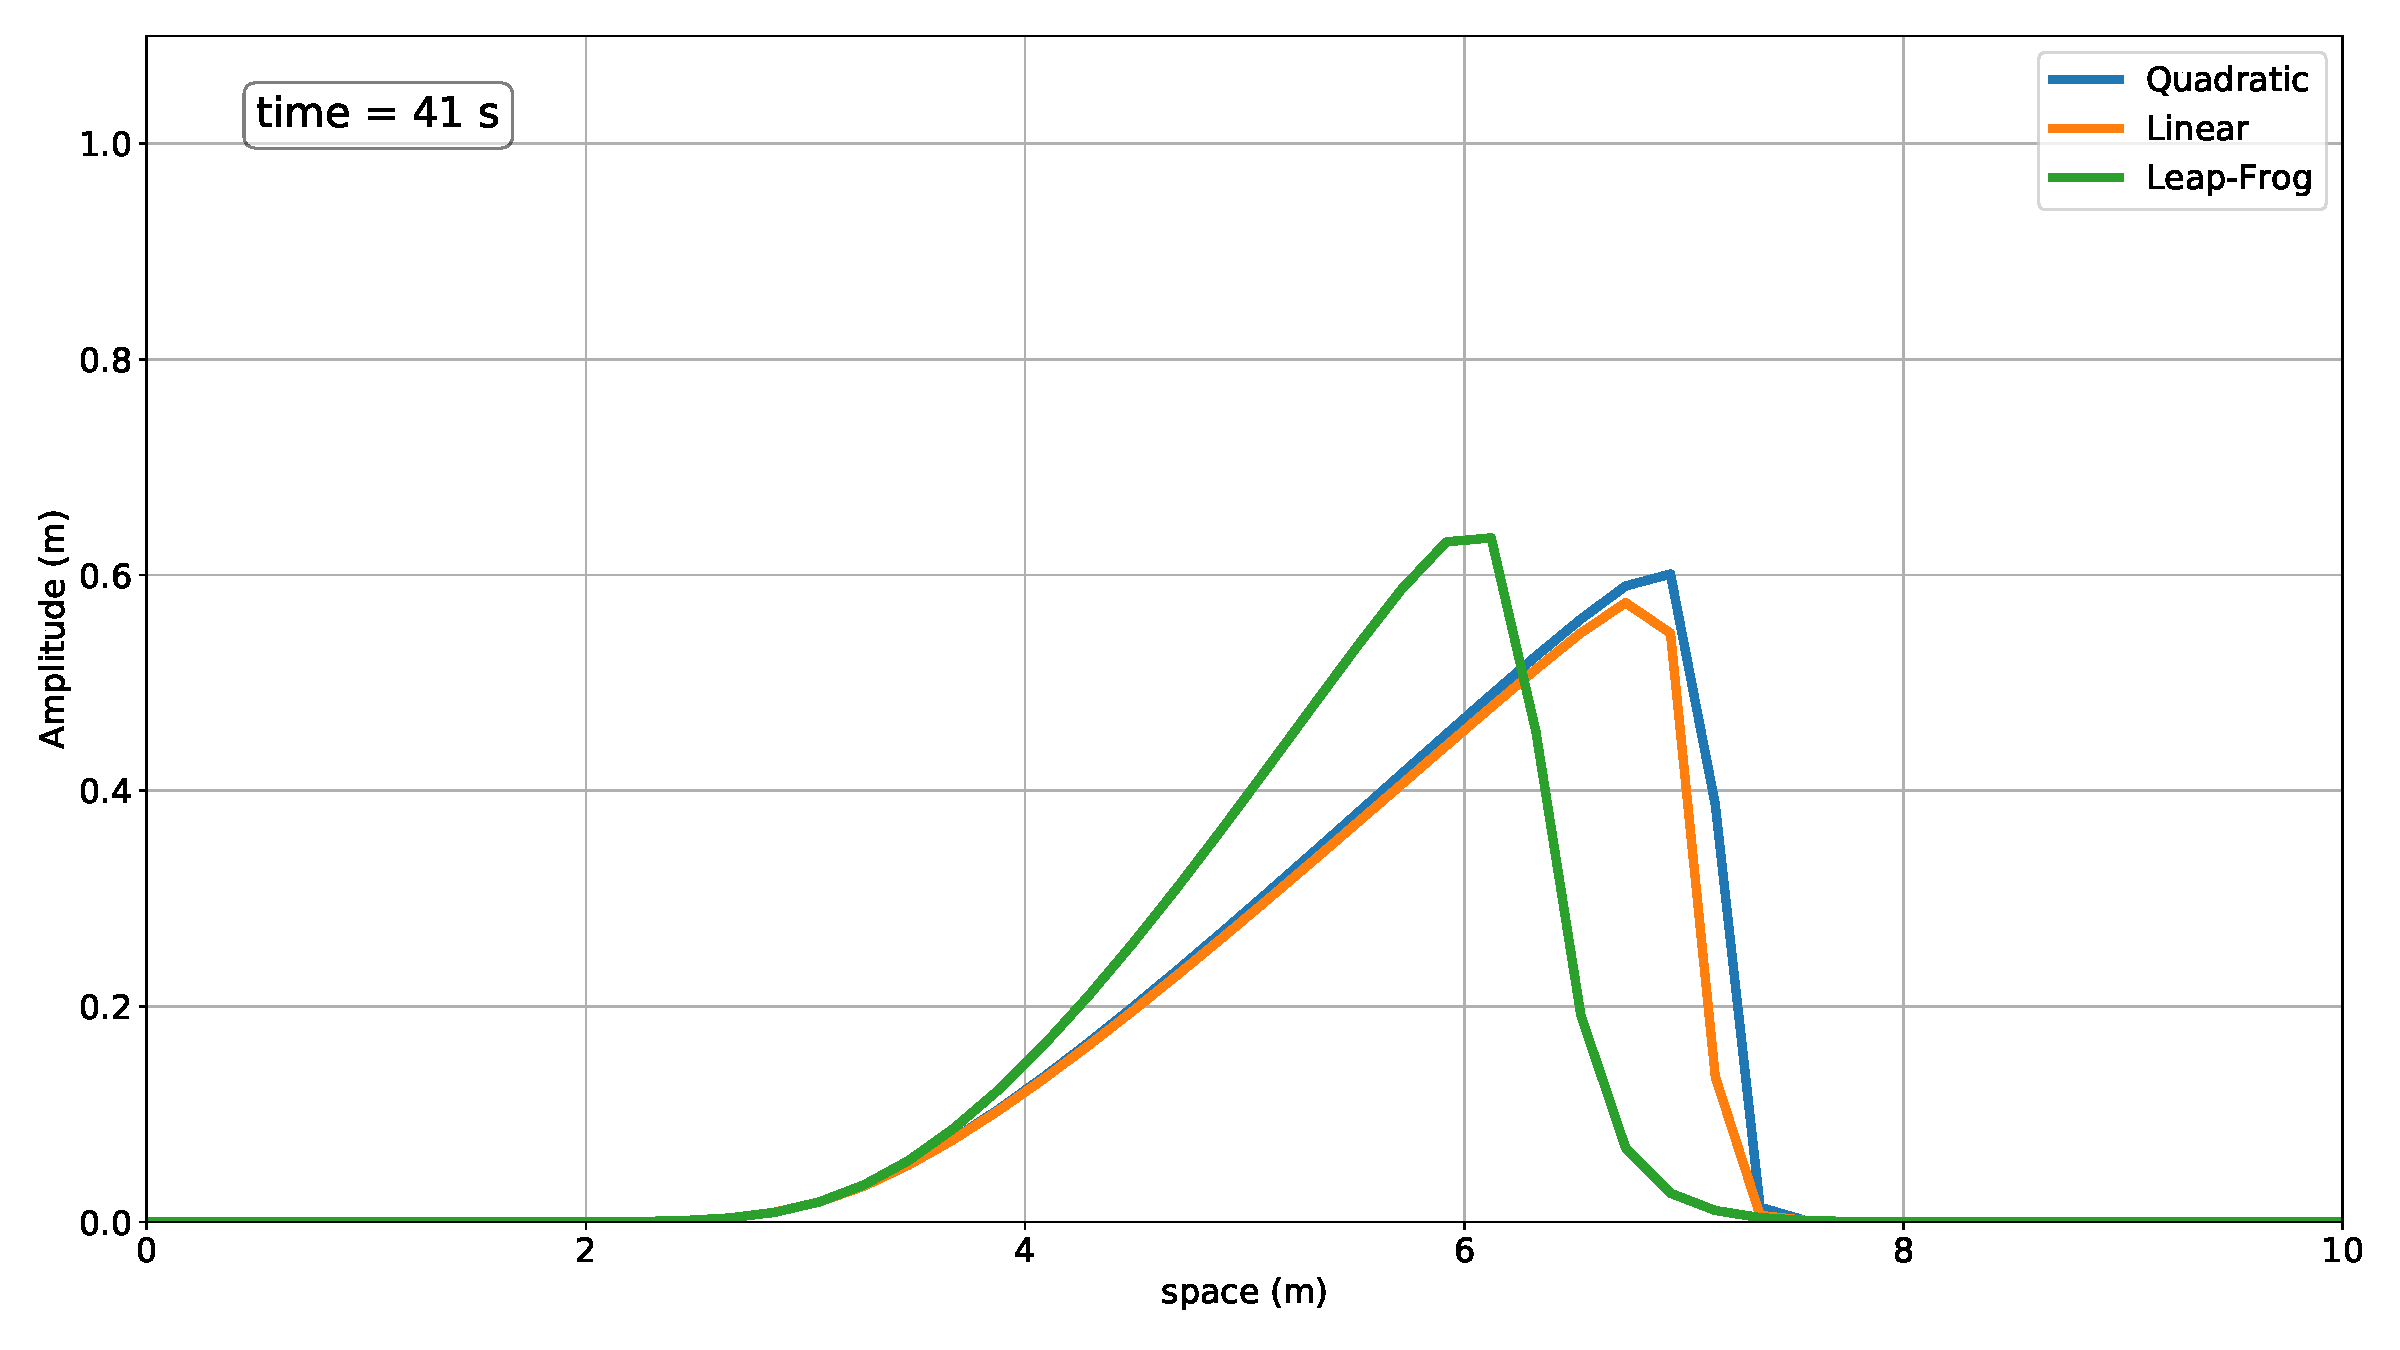
\includegraphics[width=\linewidth]{../BurgersEquation/images/imp8.pdf}
% 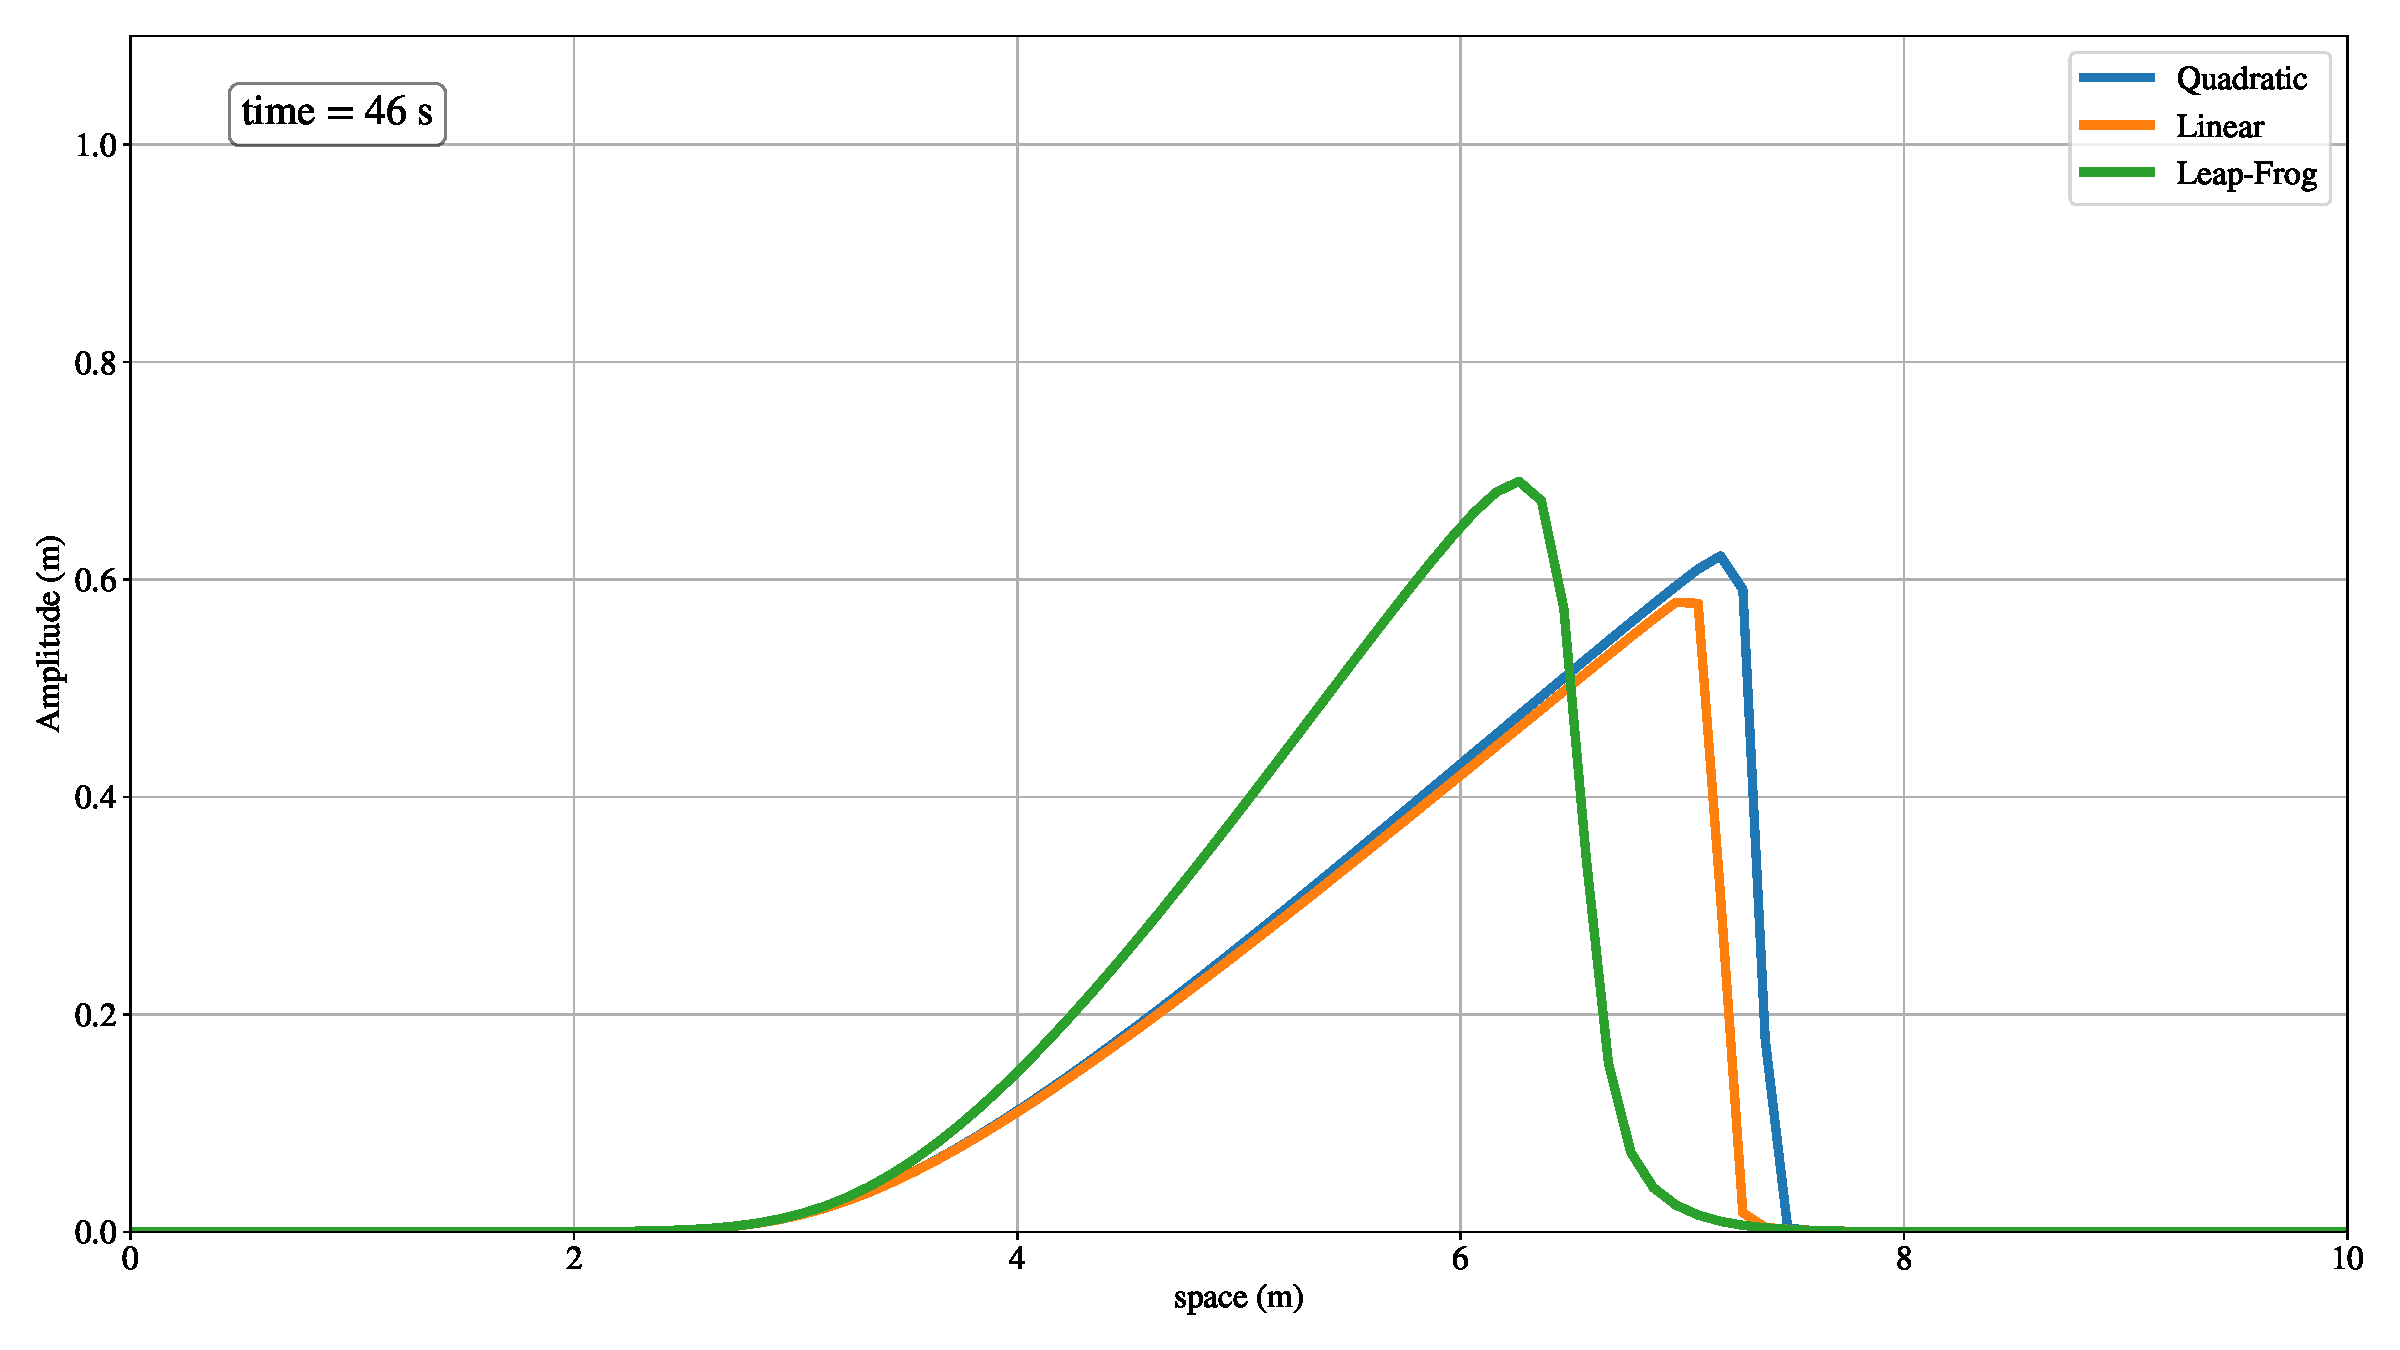
\includegraphics[width=\linewidth]{../BurgersEquation/images/imp9.pdf}
% 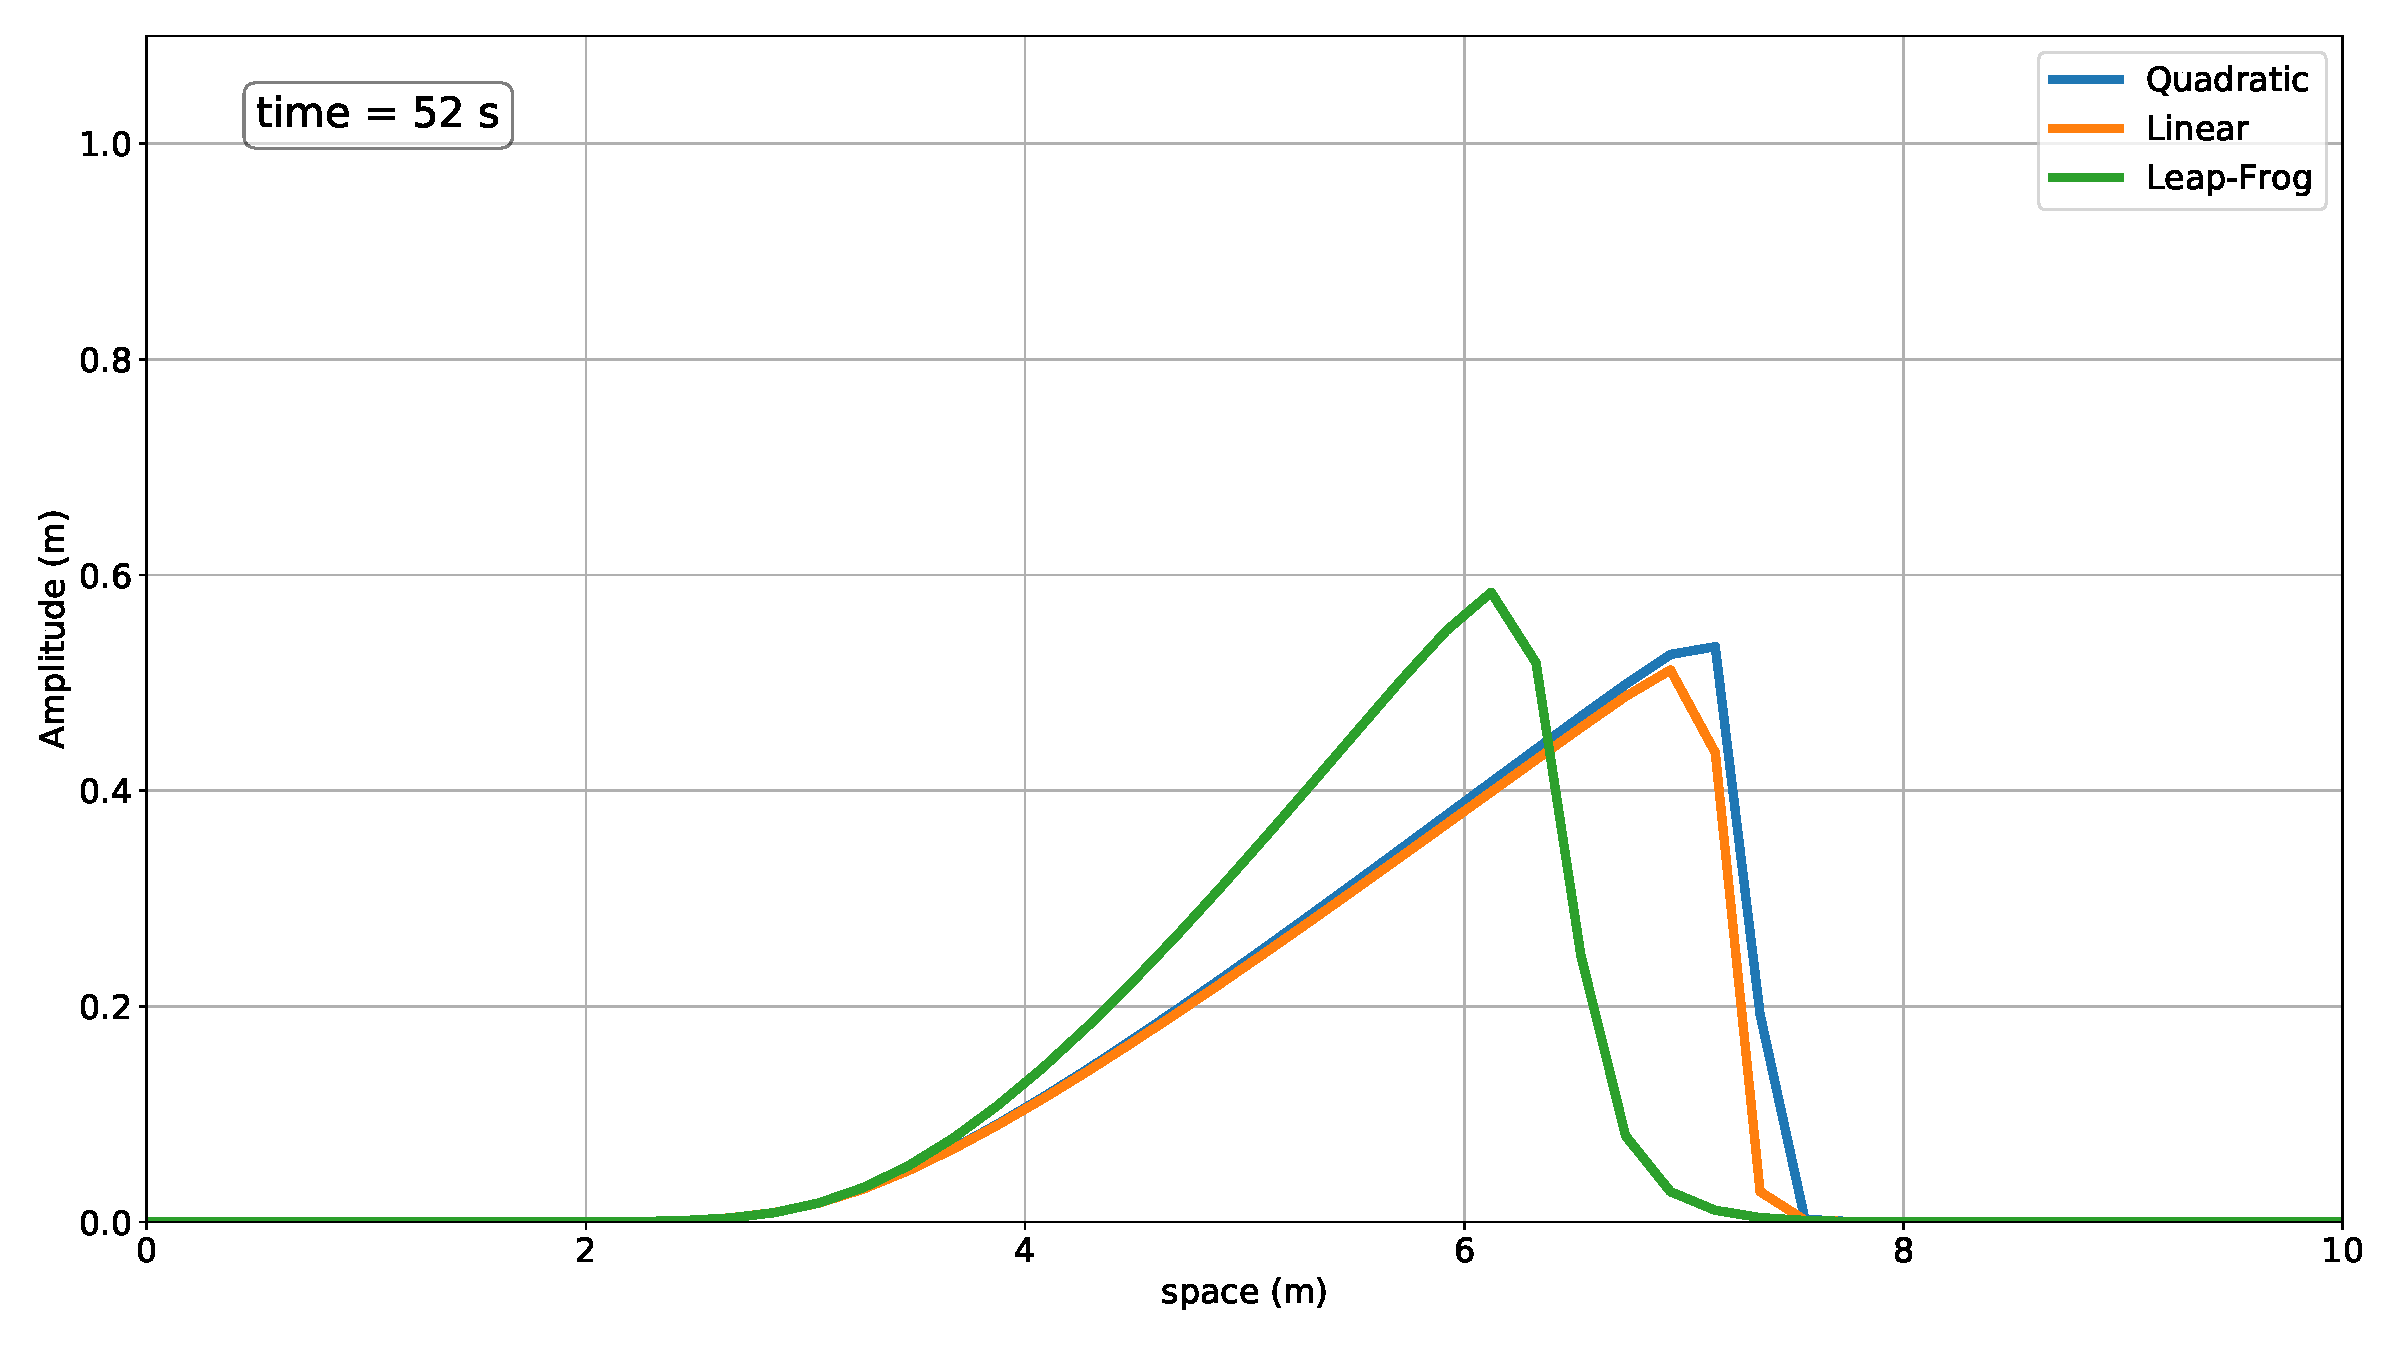
\includegraphics[width=\linewidth]{../BurgersEquation/images/imp10.pdf}
% 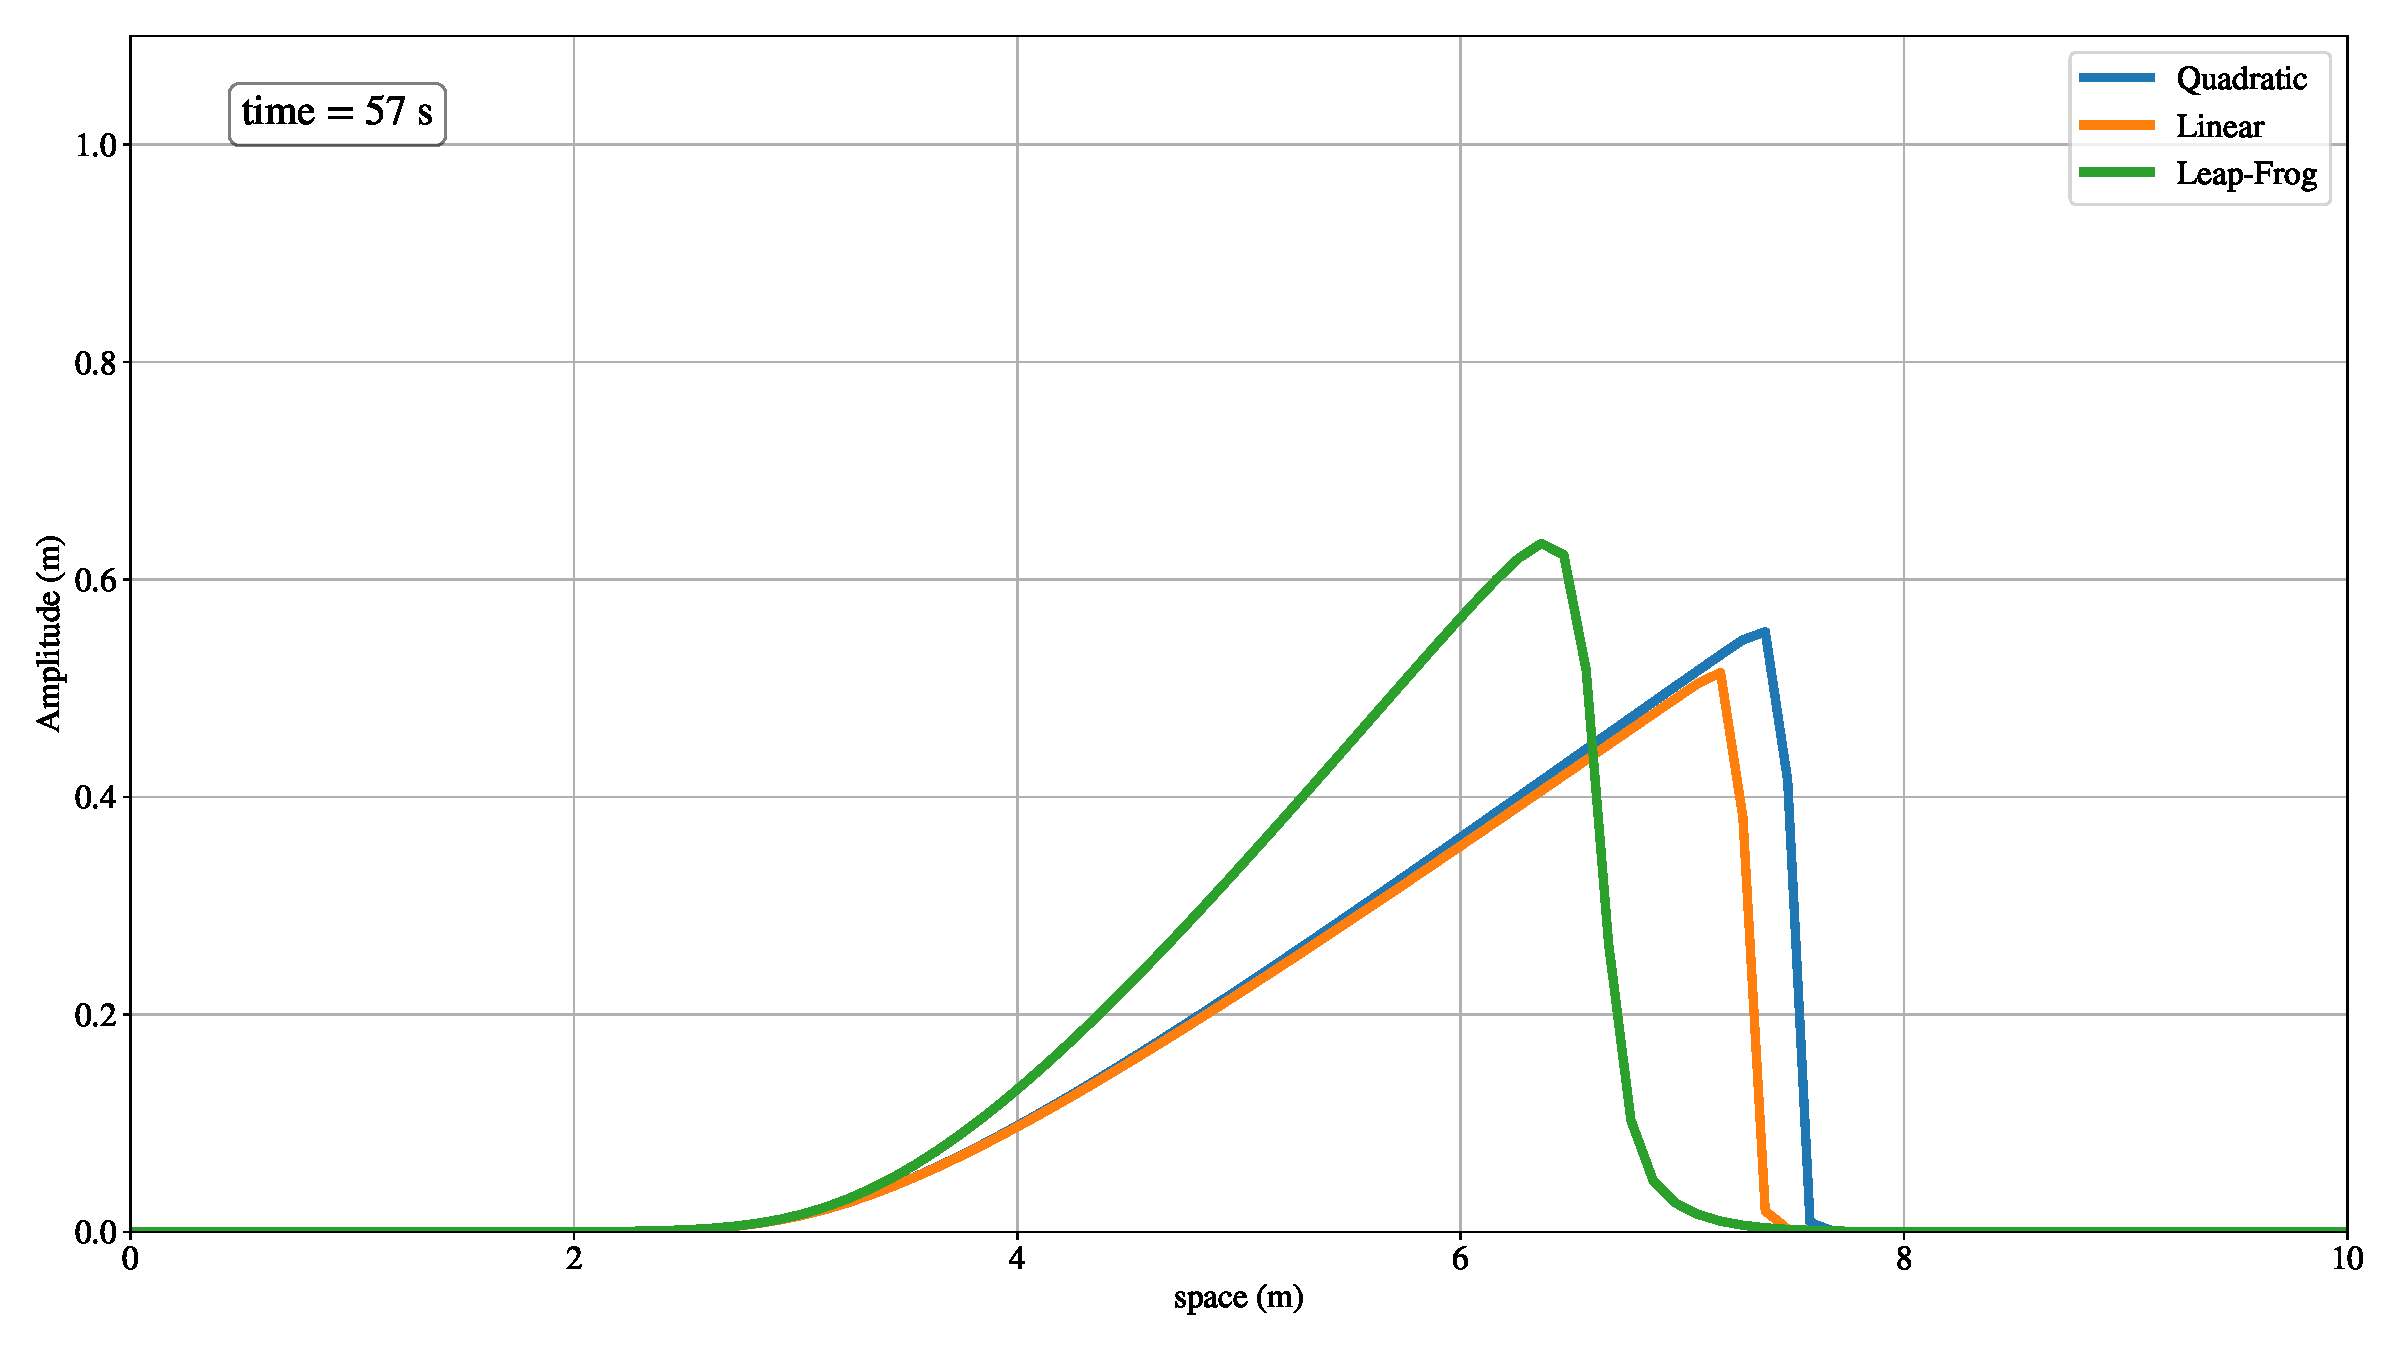
\includegraphics[width=\linewidth]{../BurgersEquation/images/imp11.pdf}
% 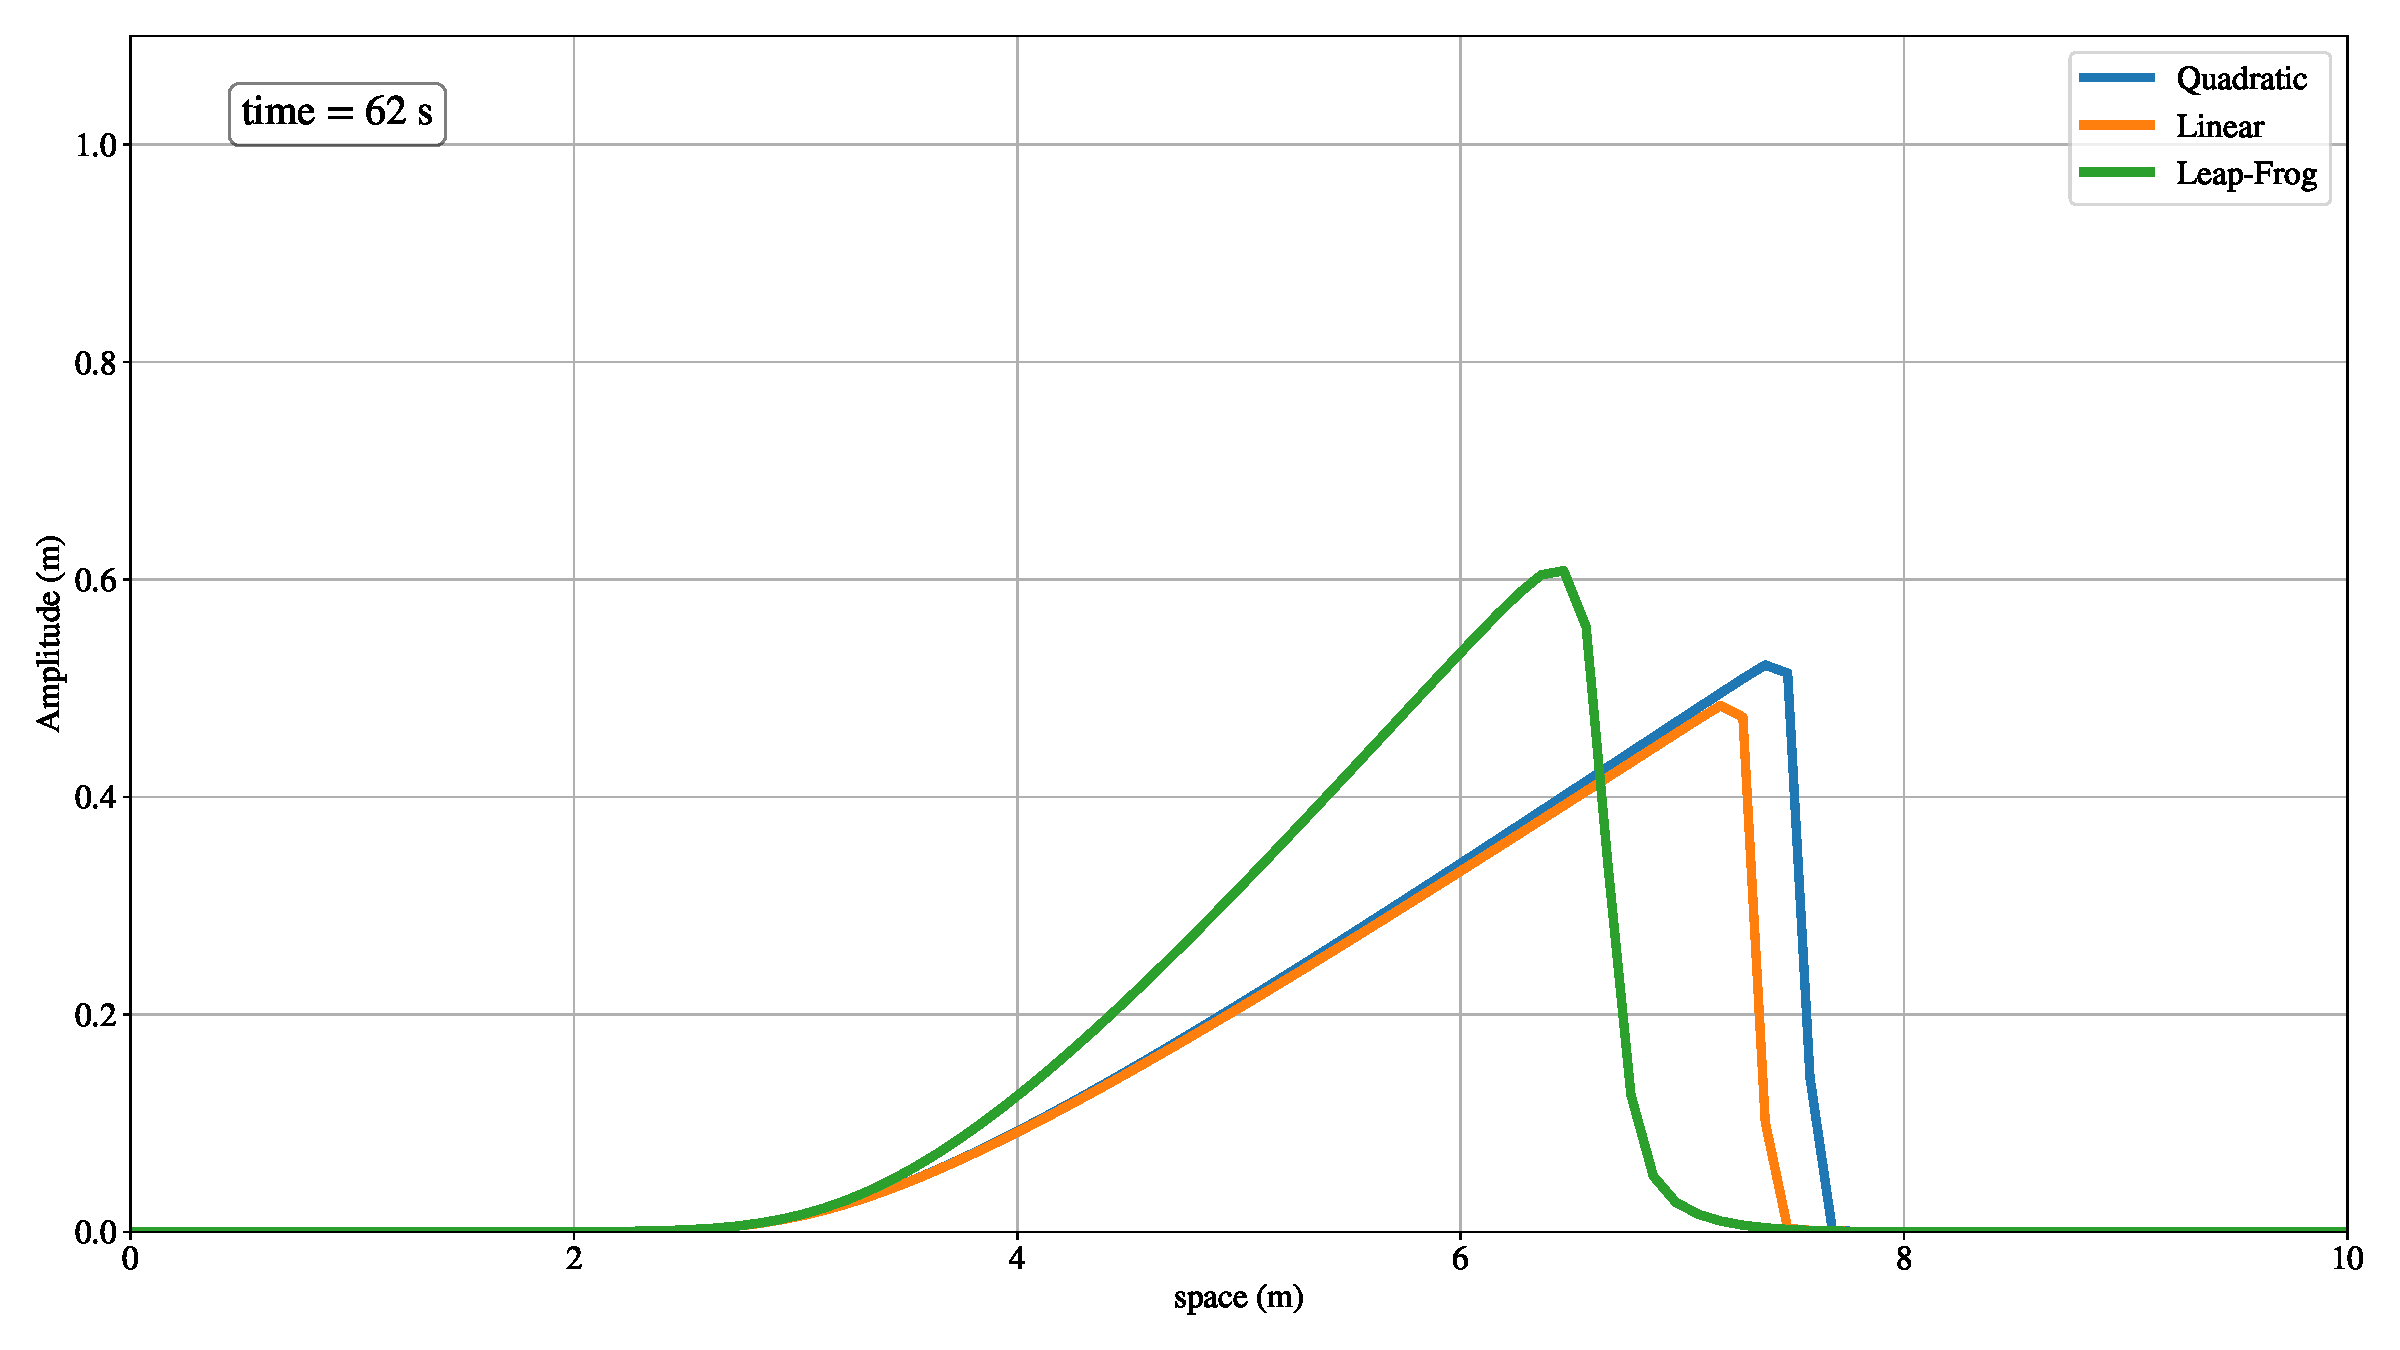
\includegraphics[width=\linewidth]{../BurgersEquation/images/imp12.pdf}
% 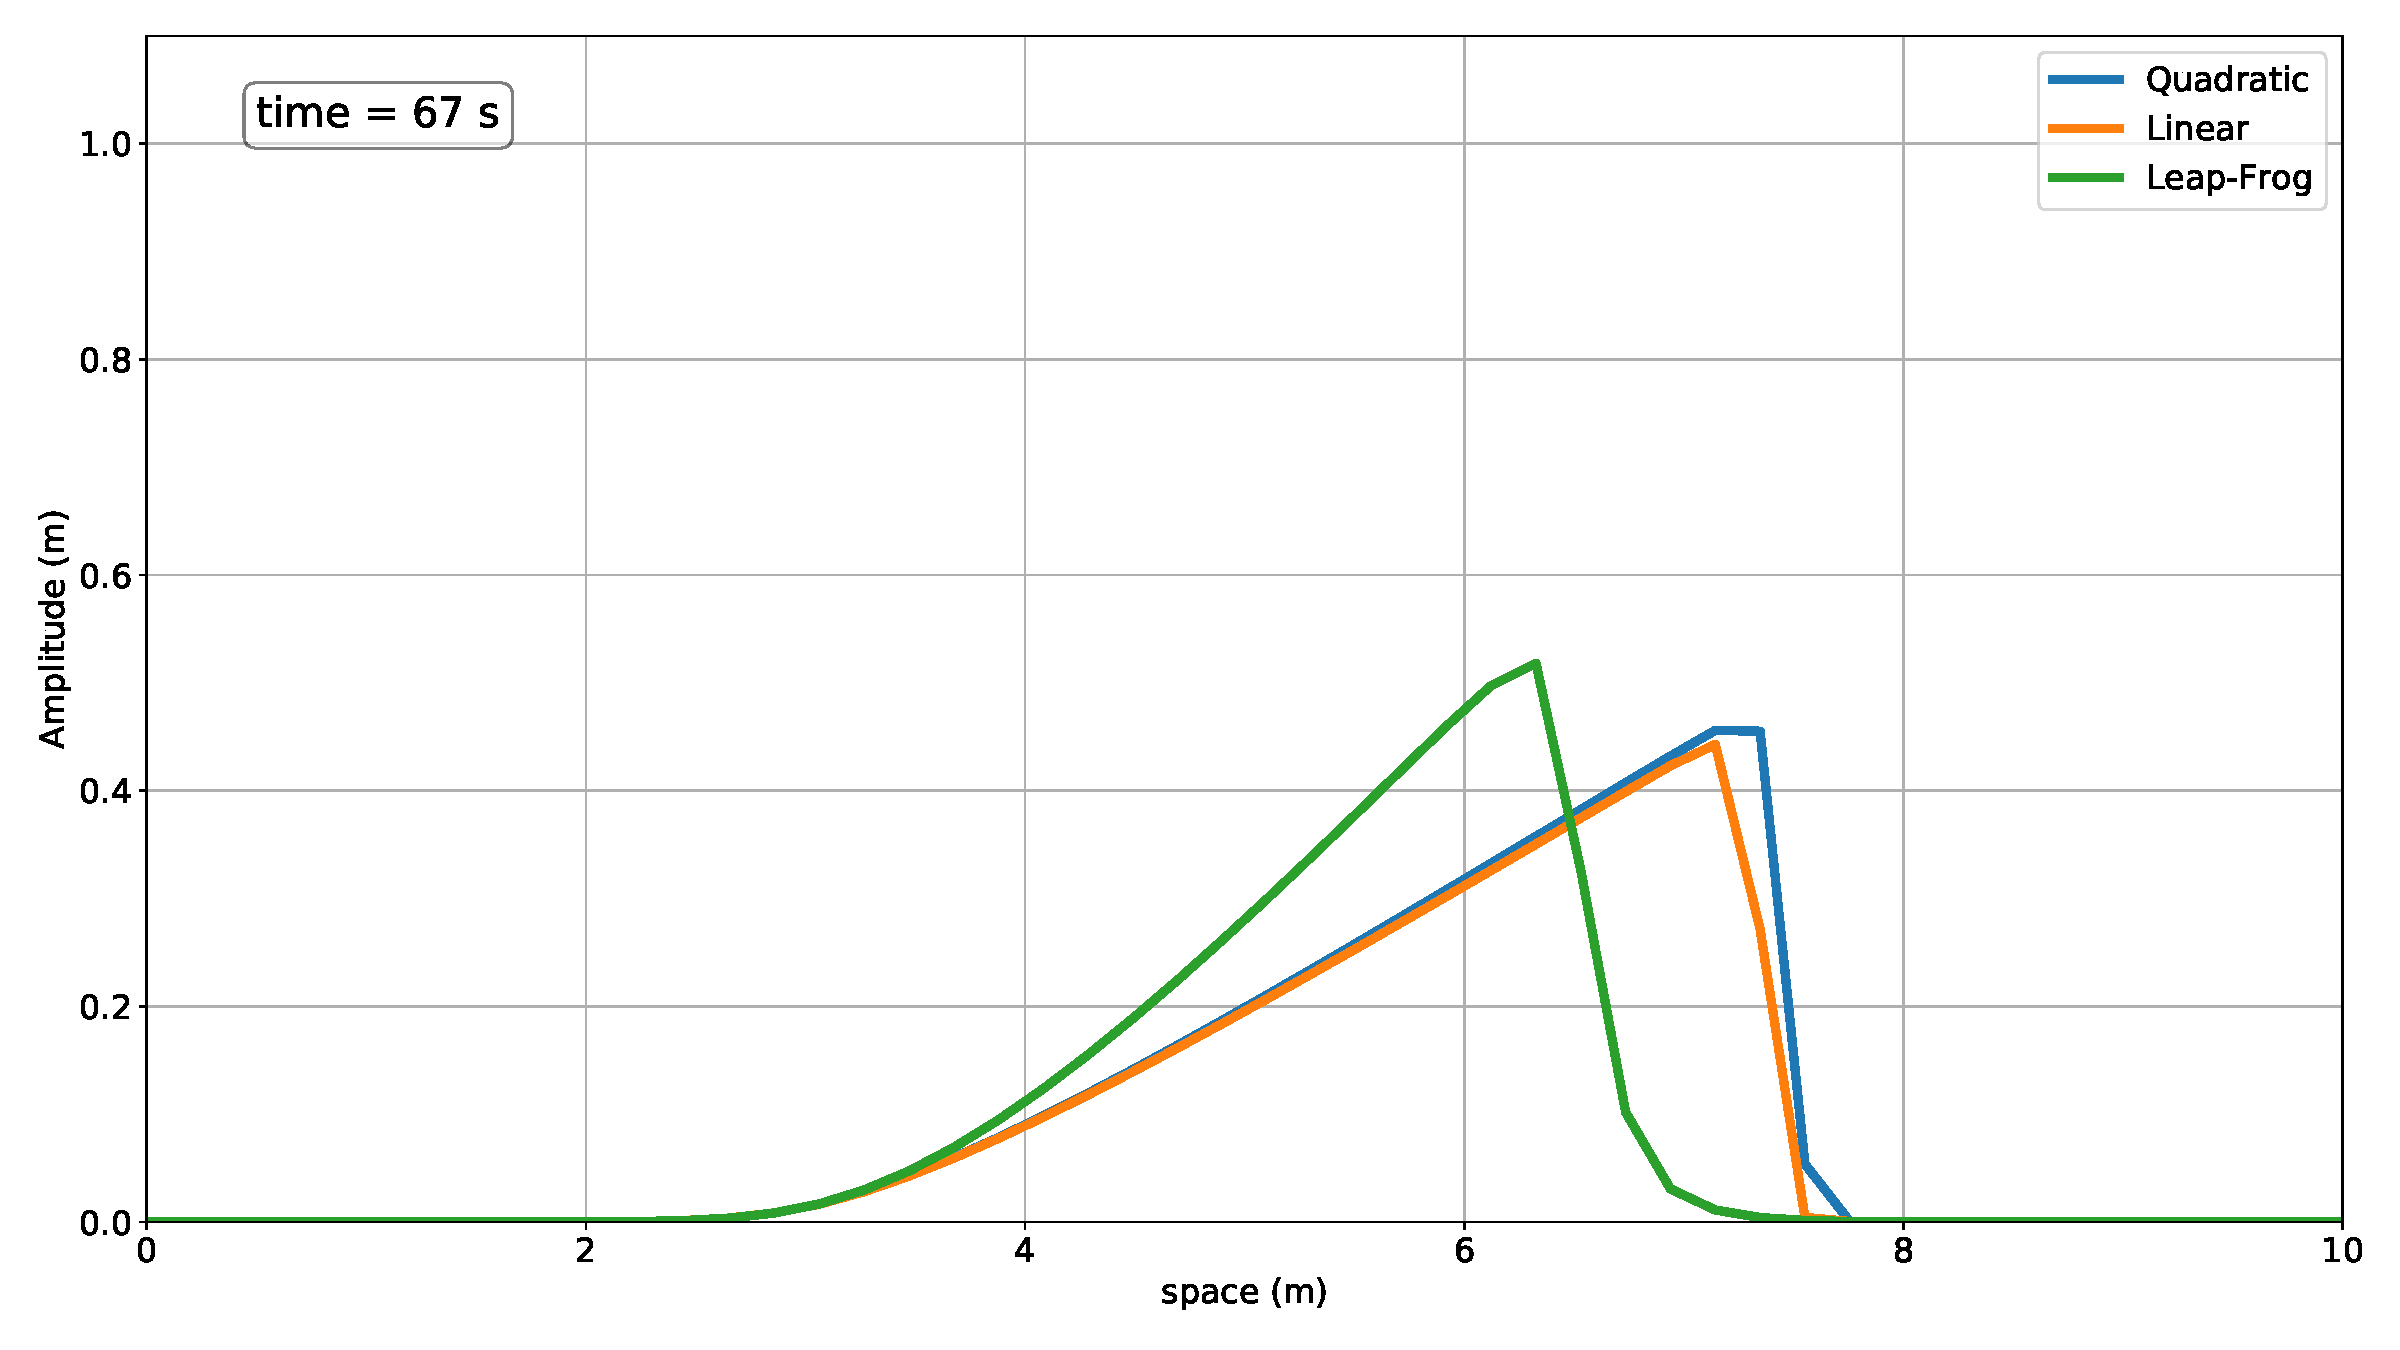
\includegraphics[width=\linewidth]{../BurgersEquation/images/imp13.pdf}
% 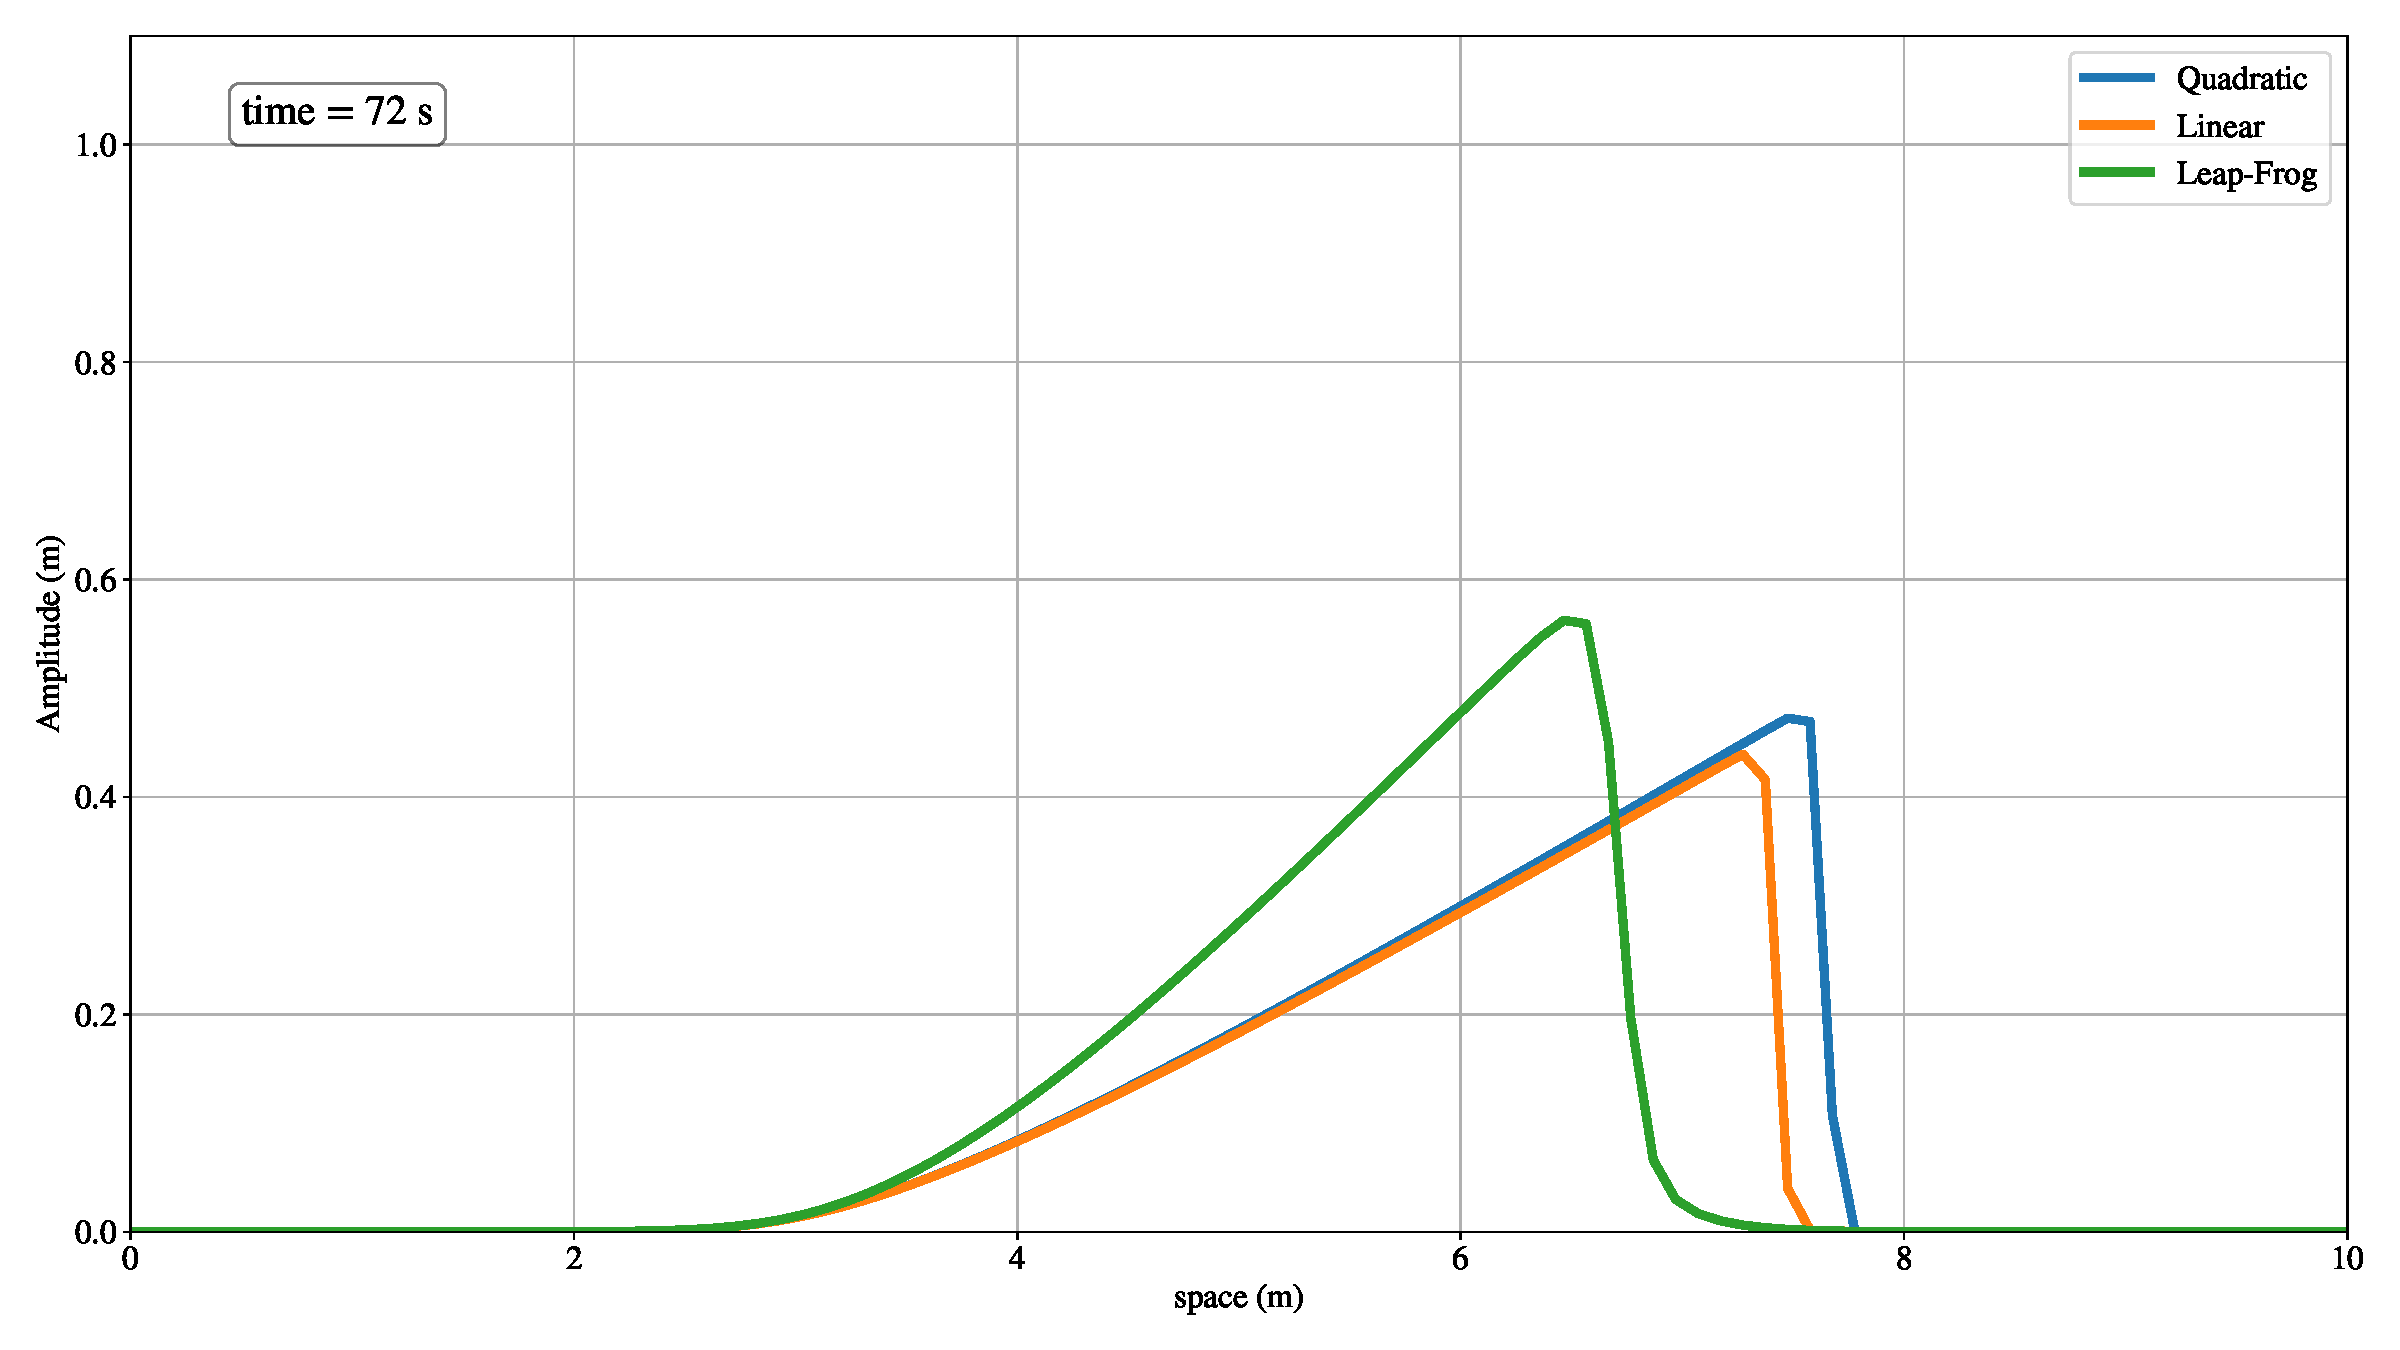
\includegraphics[width=\linewidth]{../BurgersEquation/images/imp14.pdf}
% 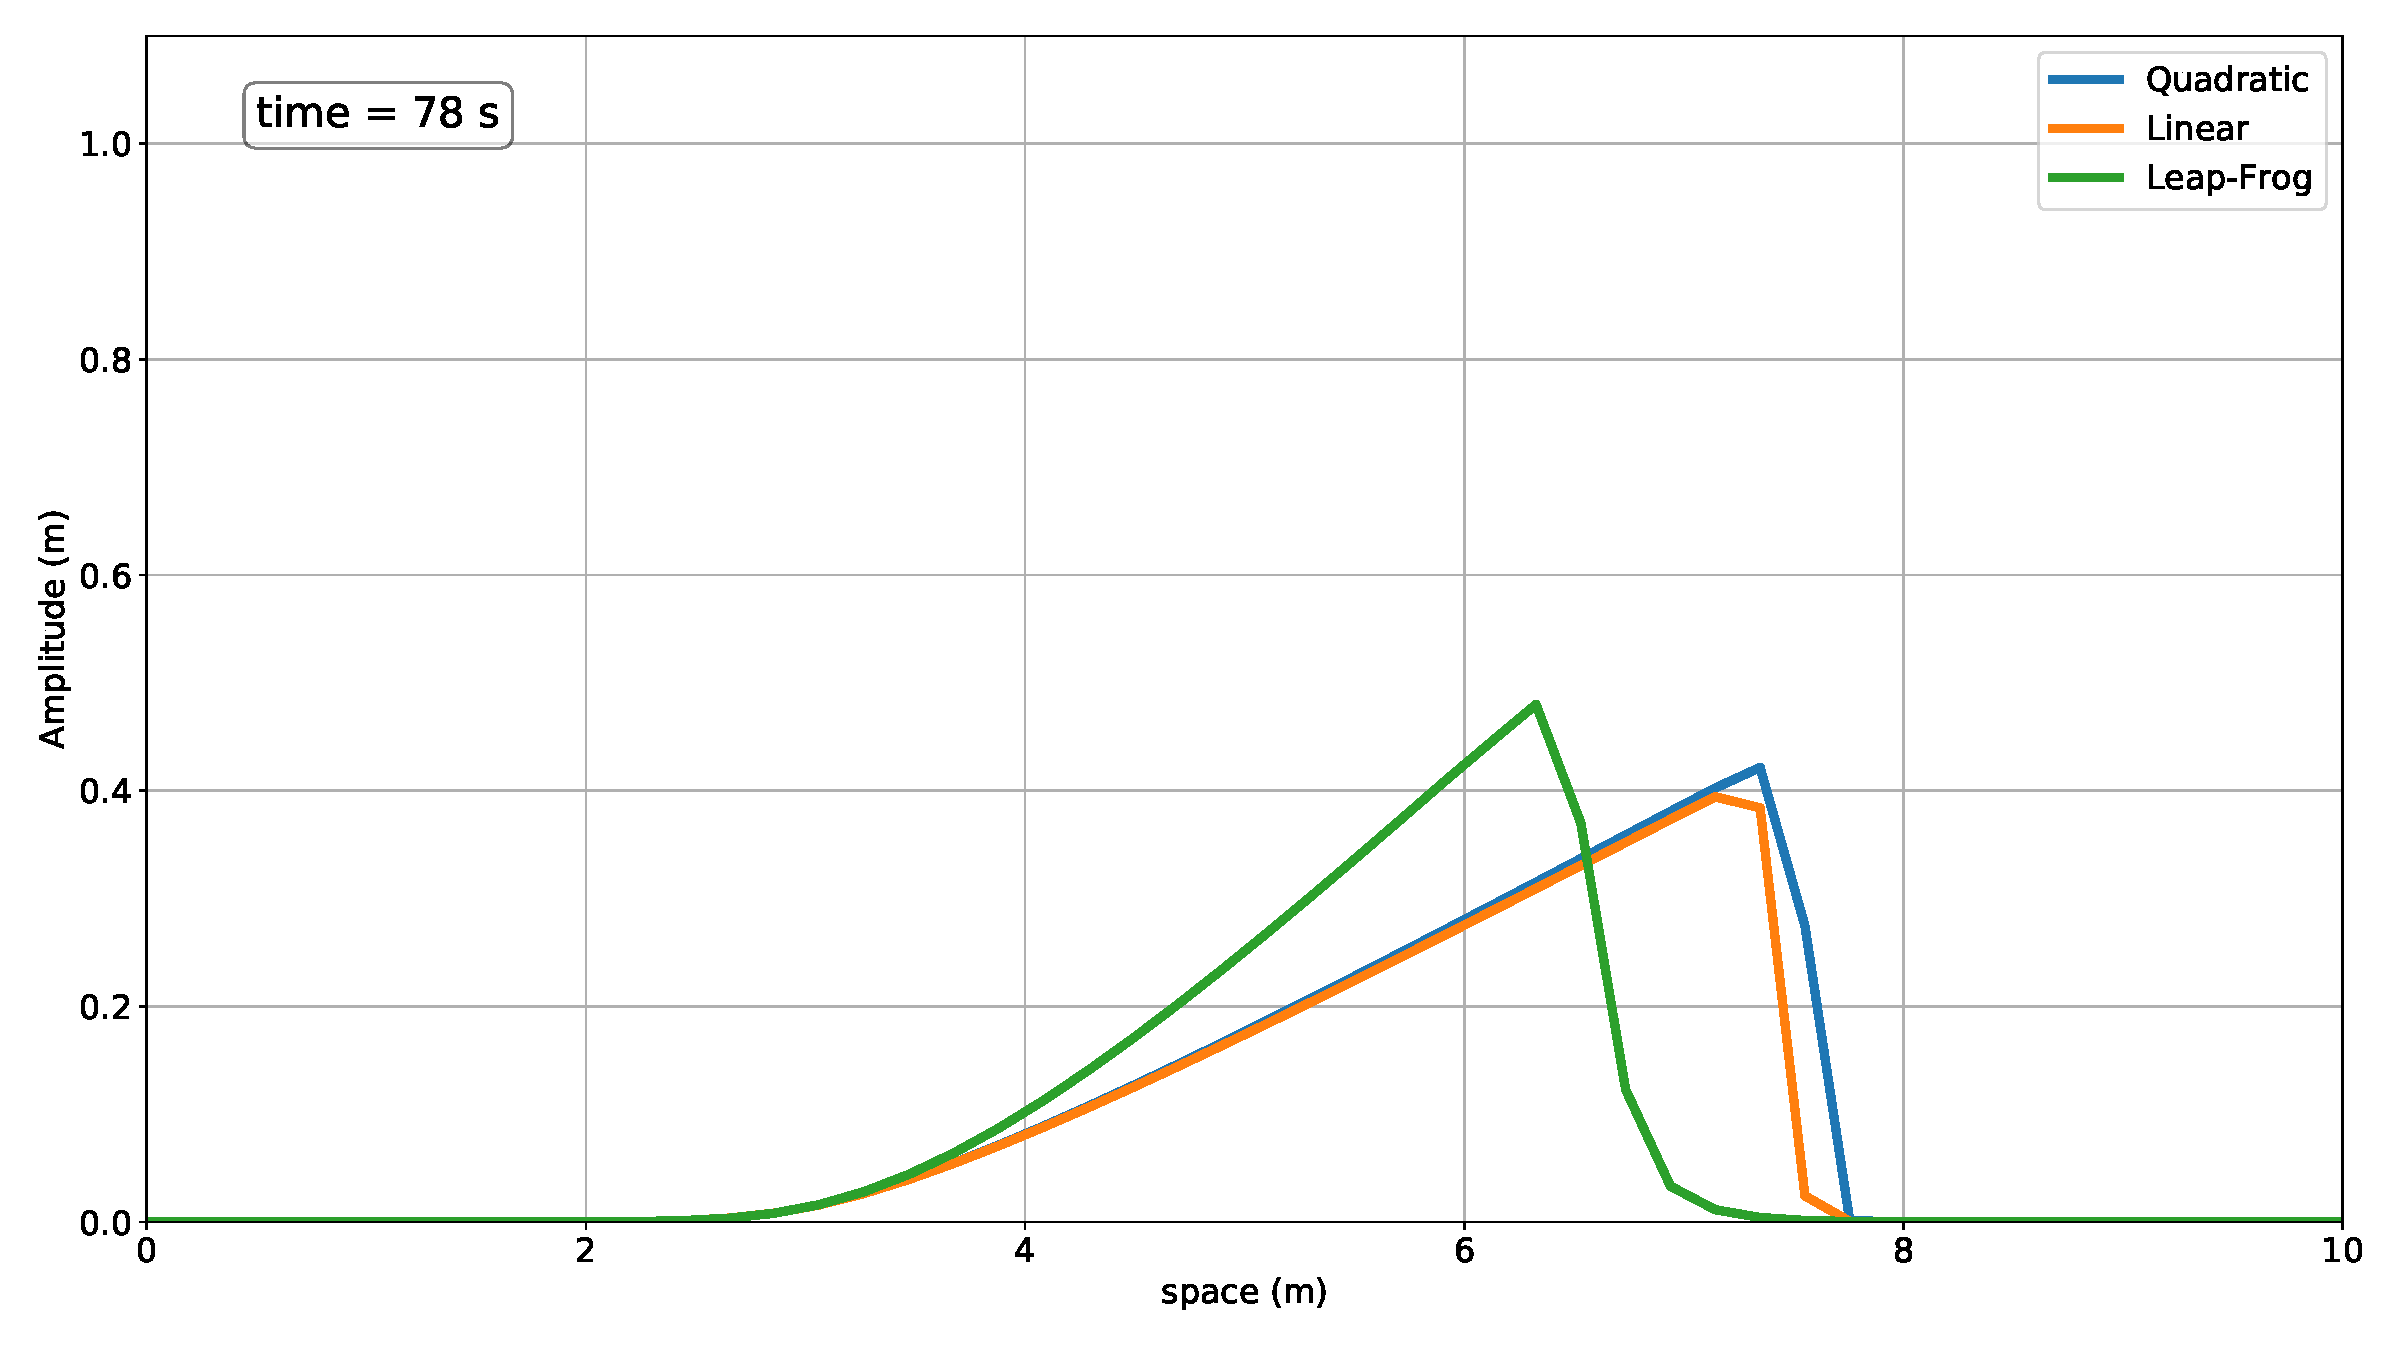
\includegraphics[width=\linewidth]{../BurgersEquation/images/imp15.pdf}
% 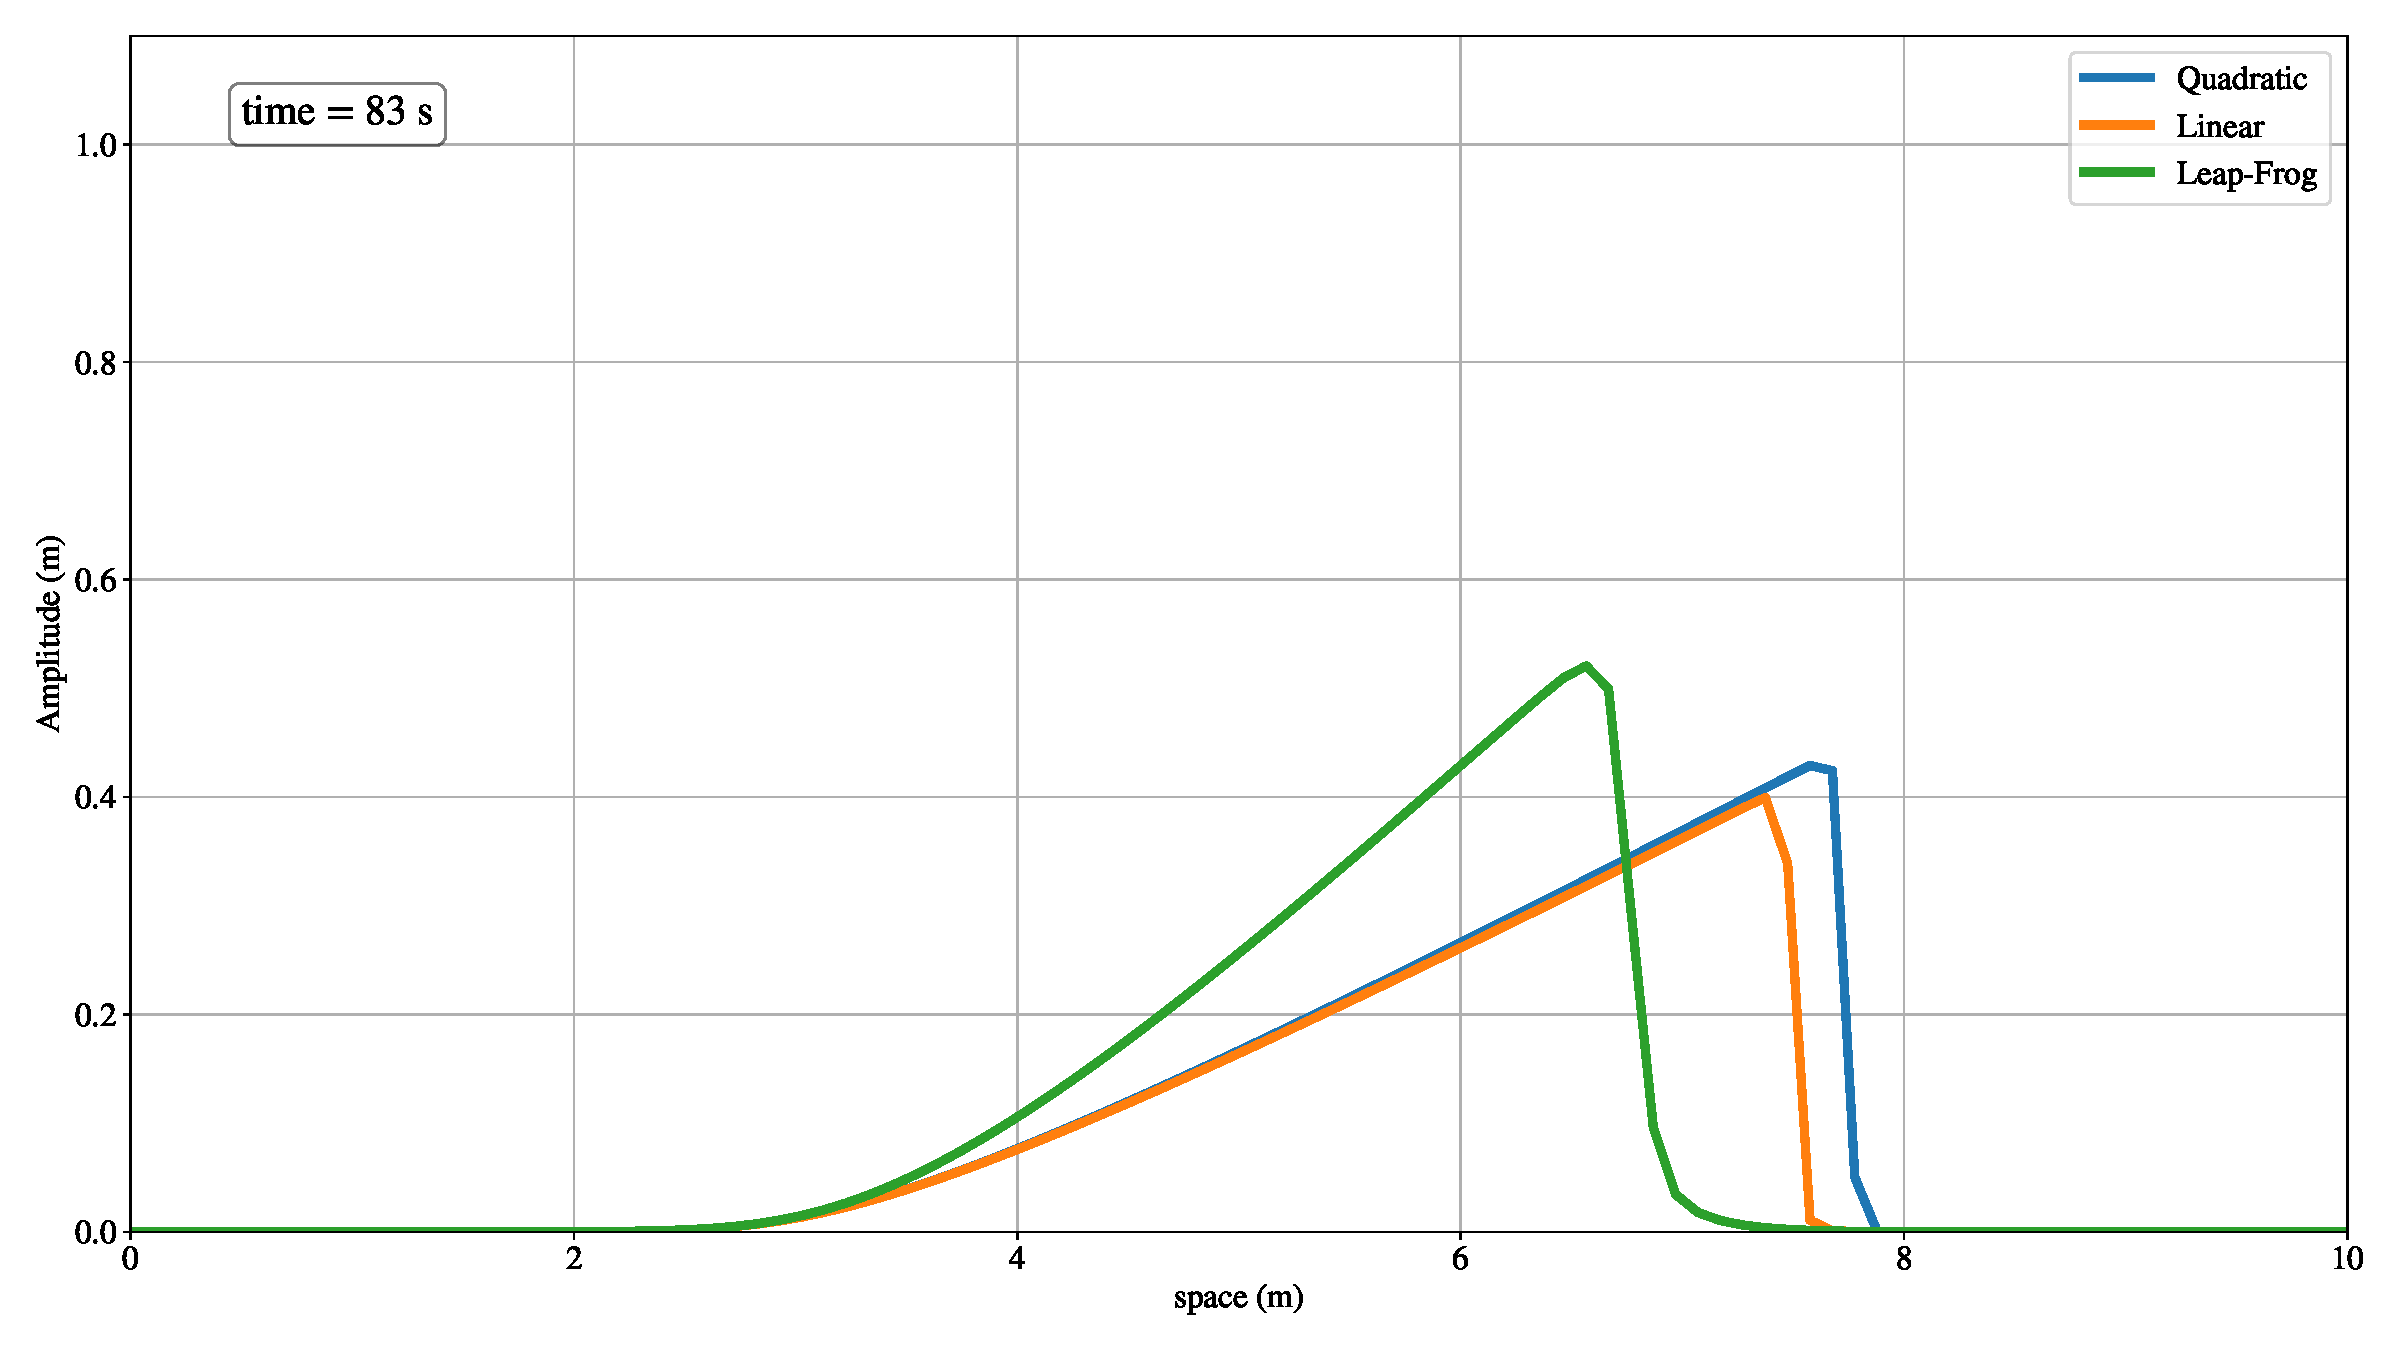
\includegraphics[width=\linewidth]{../BurgersEquation/images/imp16.pdf}
% 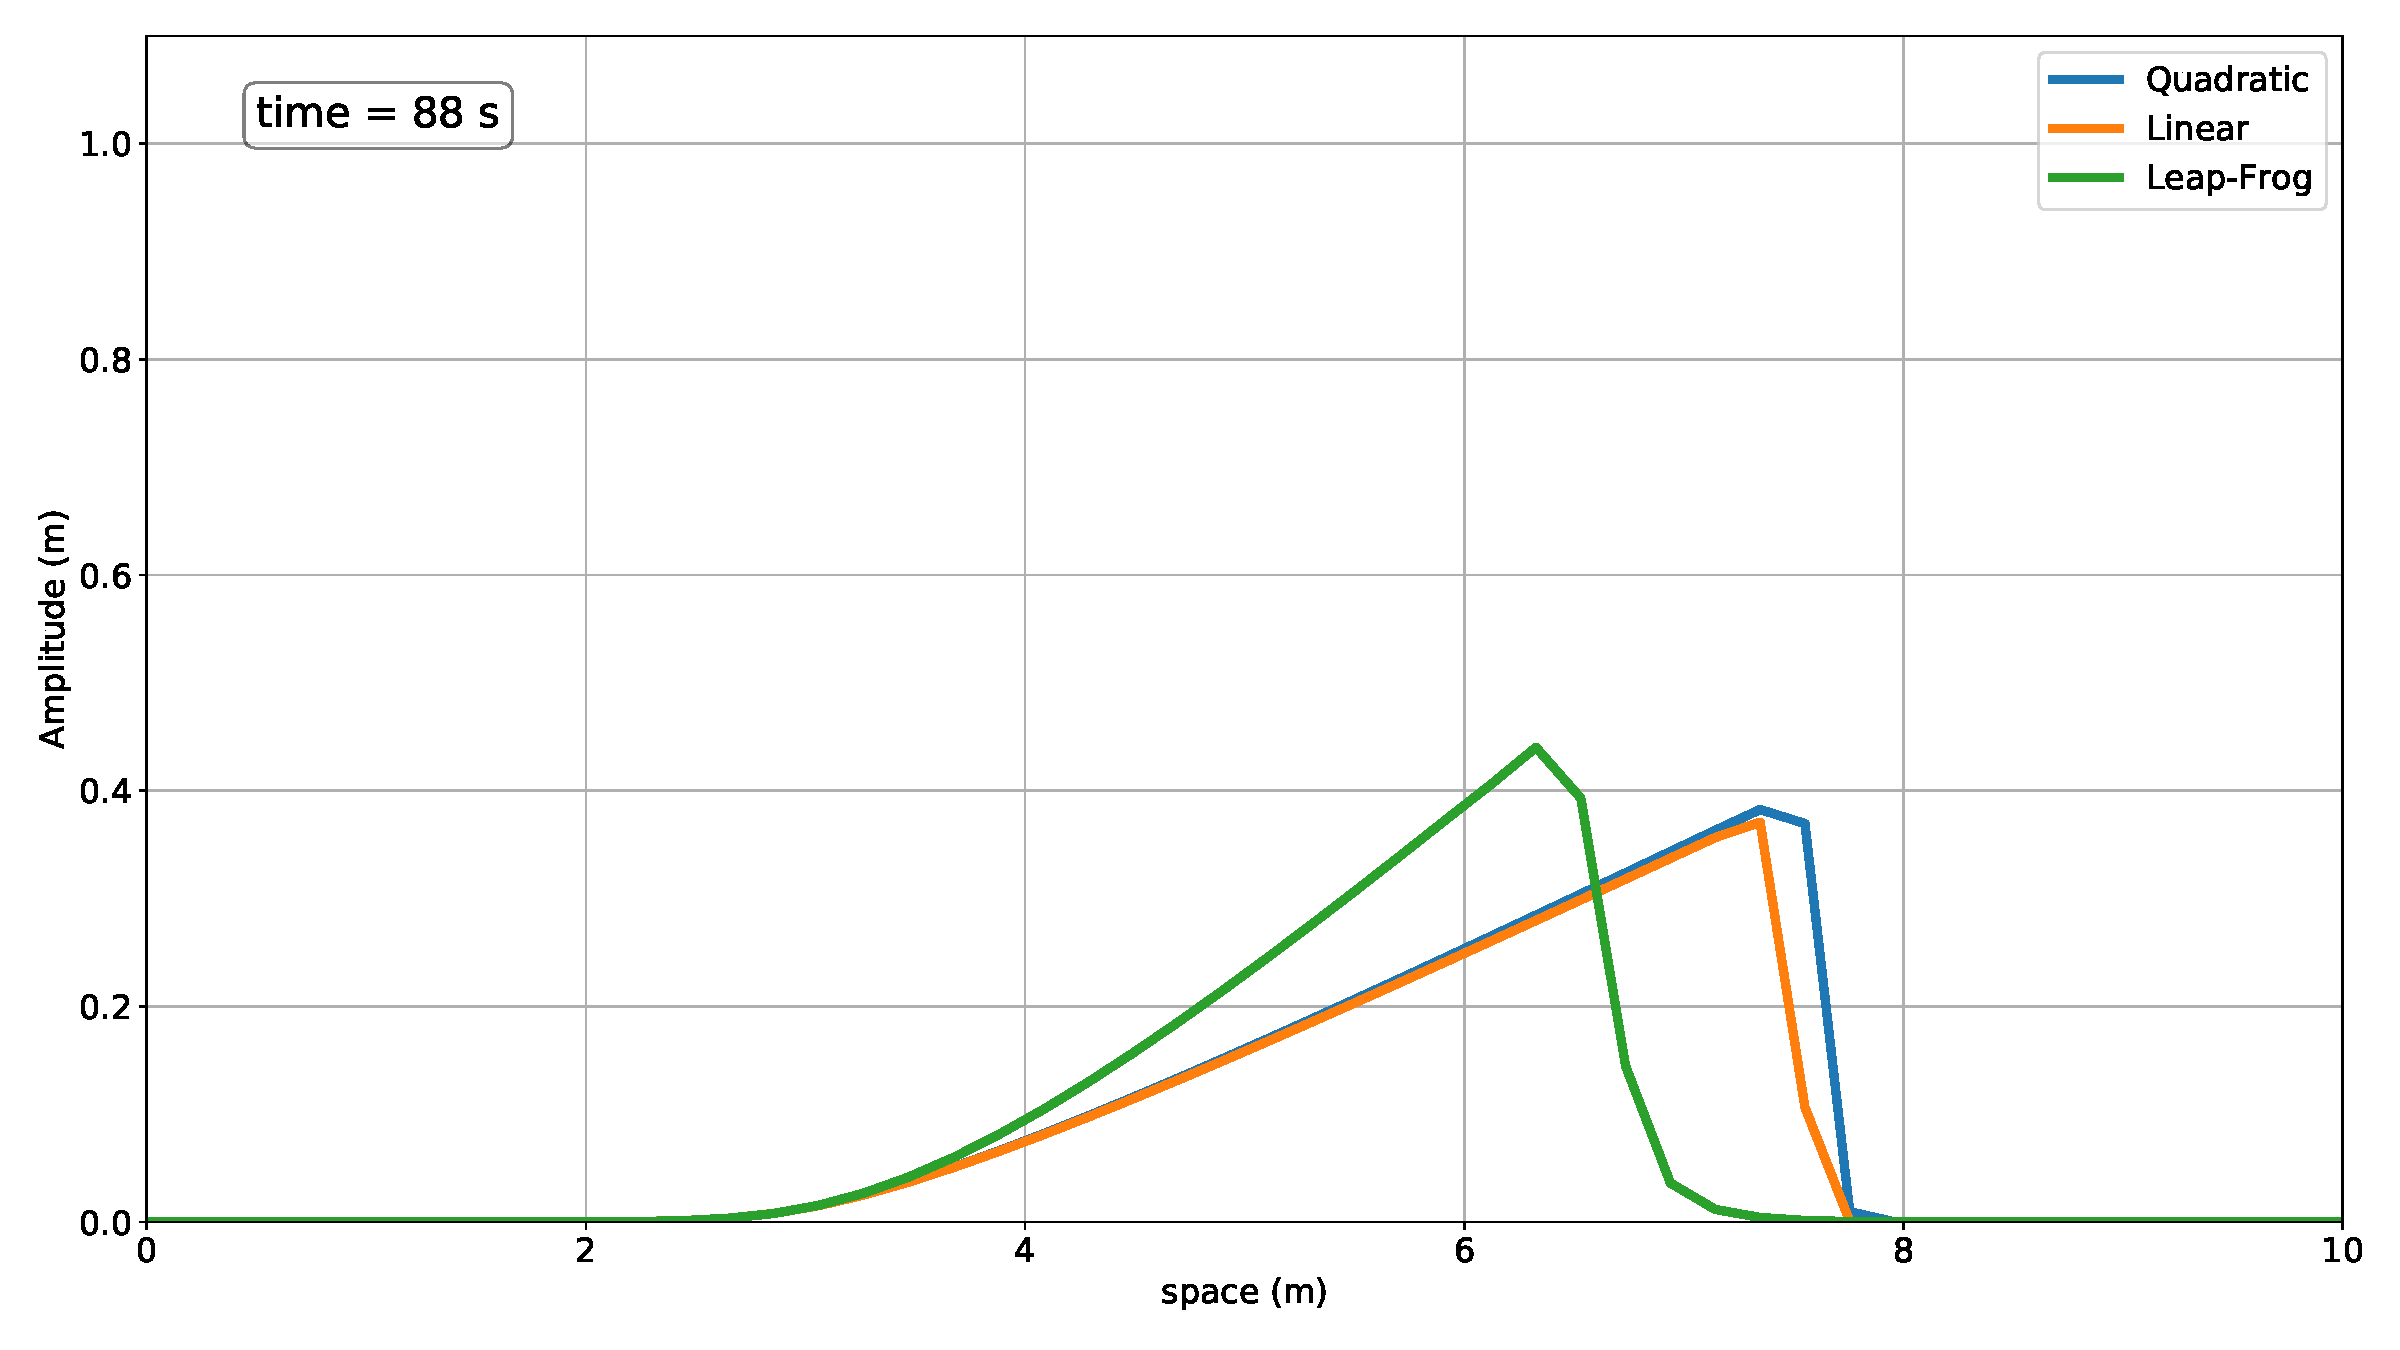
\includegraphics[width=\linewidth]{../BurgersEquation/images/imp17.pdf}
% 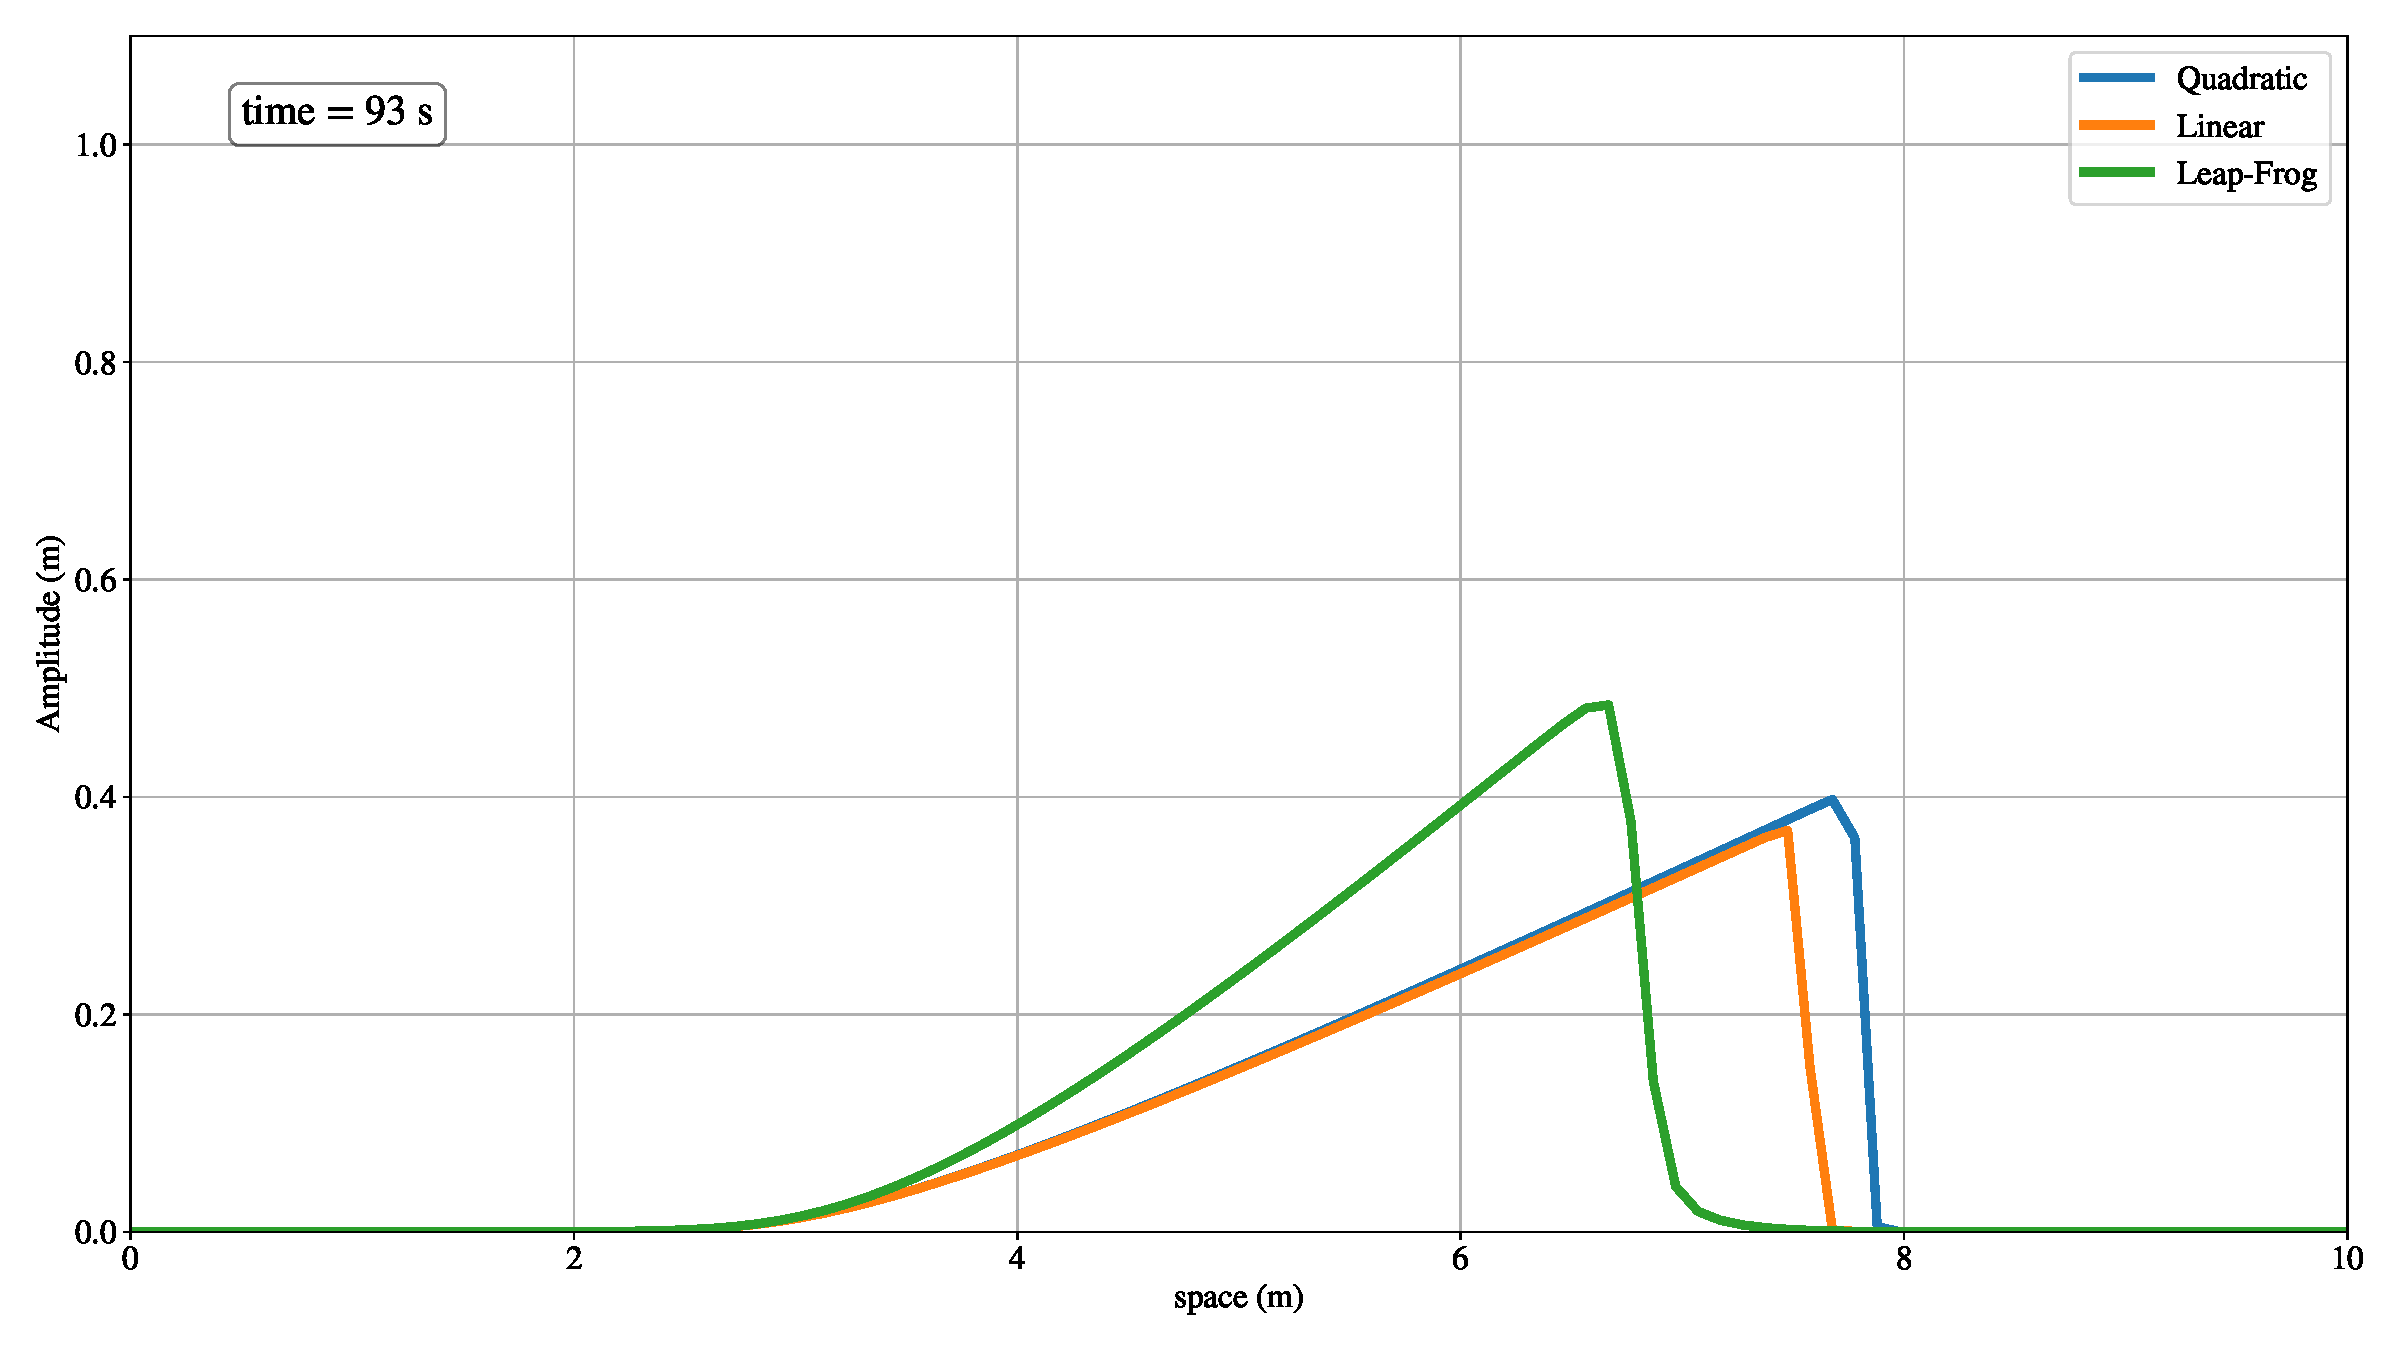
\includegraphics[width=\linewidth]{../BurgersEquation/images/imp18.pdf}
% 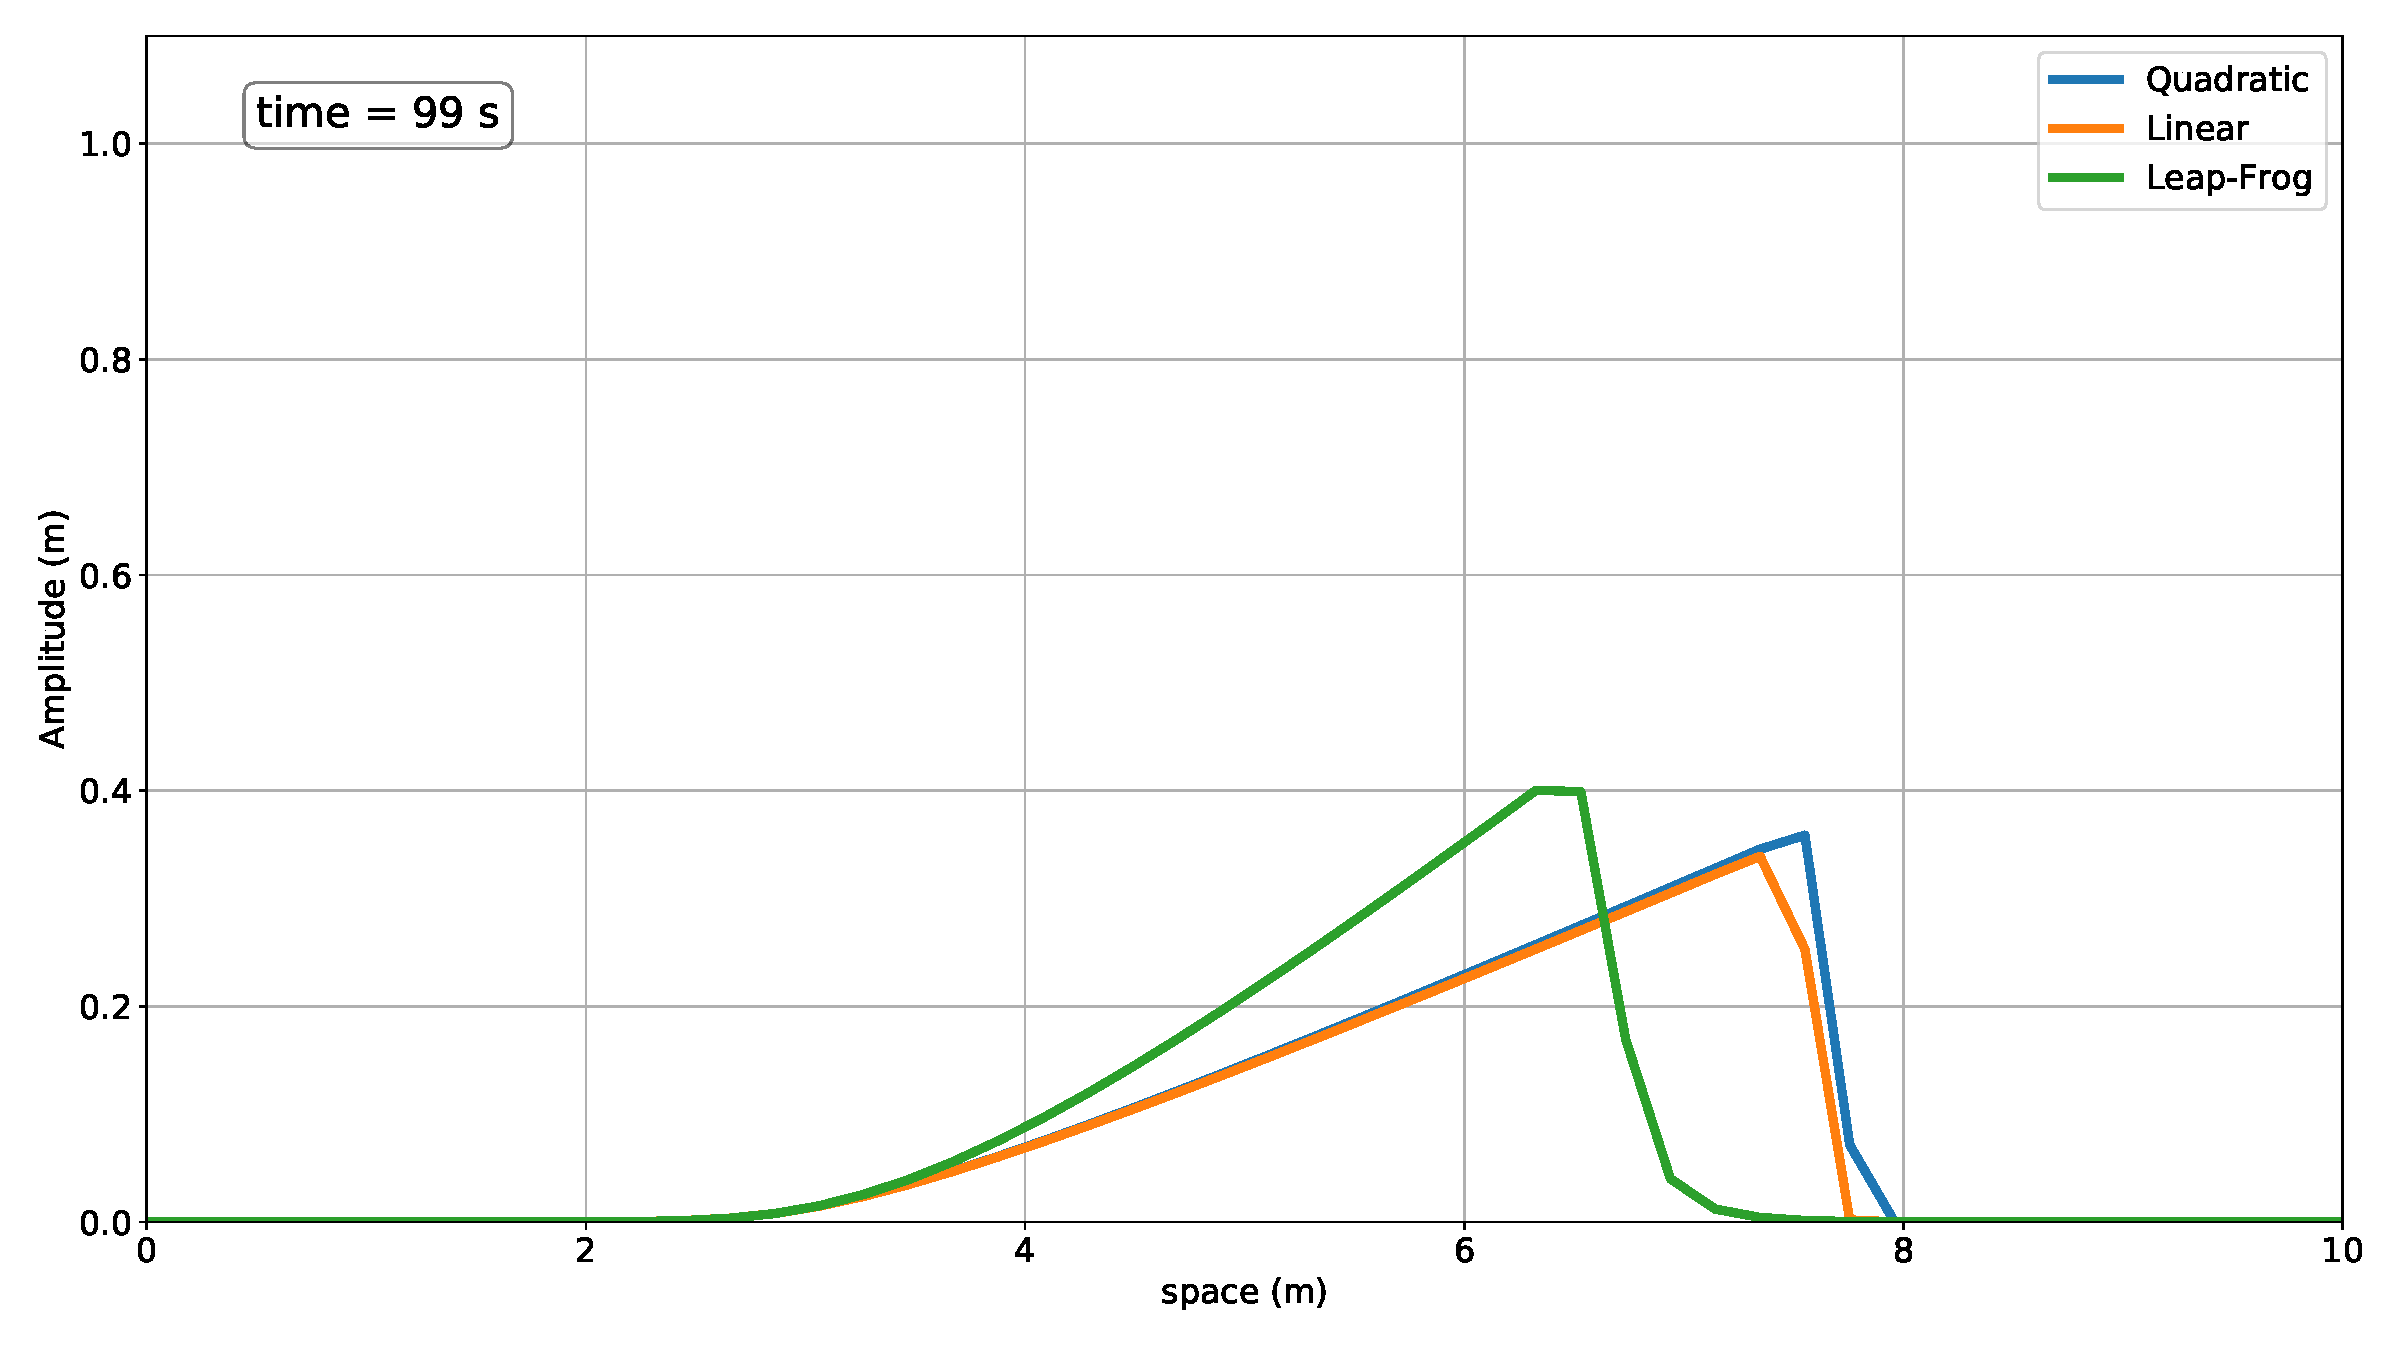
\includegraphics[width=\linewidth]{../BurgersEquation/images/imp19.pdf}

\begin{frame}
  \begin{columns}
    \column{0.5\linewidth}
    \begin{center}
      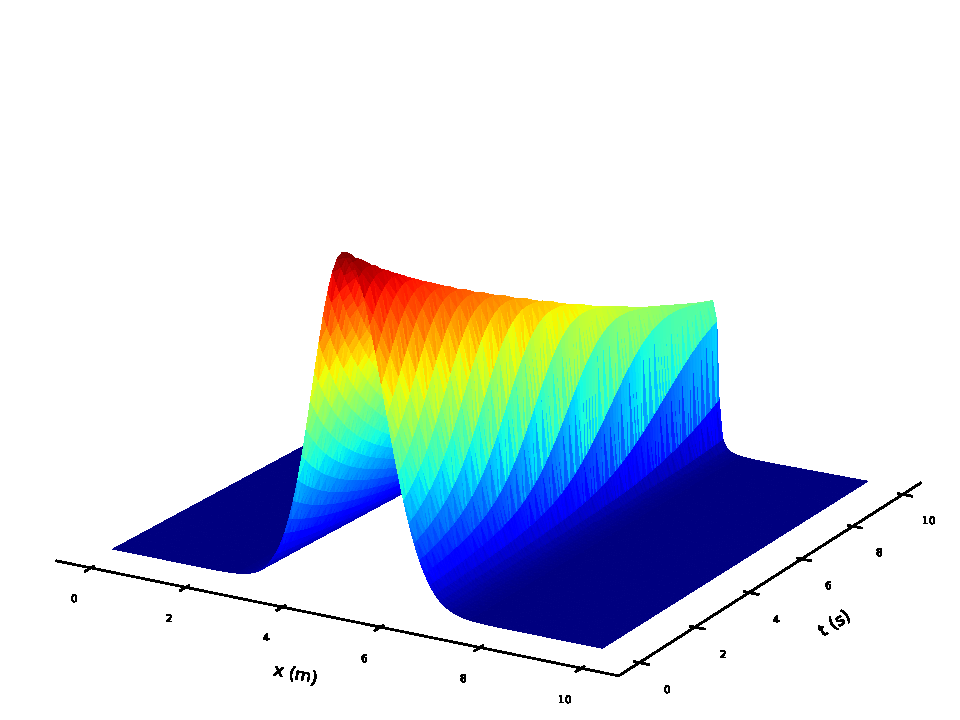
\includegraphics[height=.7\textheight]{../BurgersEquation/images/Implicit_front.pdf}
    \end{center}
    \column{0.5\linewidth}
    \begin{center}
      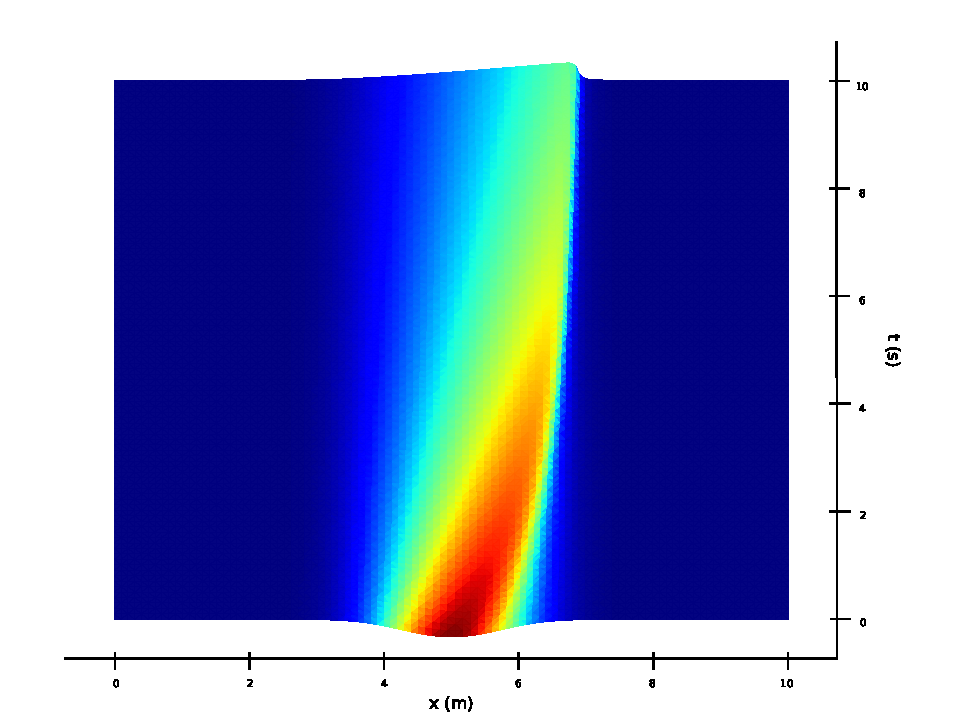
\includegraphics[height=.7\textheight]{../BurgersEquation/images/Implicit_top.pdf}
    \end{center}
  \end{columns}
\end{frame}

\begin{frame}
  \frametitle{Convergence Condition}
  Stable!
\end{frame}
